\documentclass[11pt,letterpaper]{article}

\usepackage{amsmath,amssymb}
\usepackage{graphicx}
\usepackage{booktabs}
\usepackage{enumitem}
\usepackage[margin=1in]{geometry}
\usepackage[hidelinks]{hyperref}
\usepackage{xcolor}
\usepackage{caption}
\usepackage{subcaption}
\usepackage{array}

\hypersetup{
  colorlinks=true,
  linkcolor=blue!45!black,
  citecolor=blue!45!black,
  urlcolor=blue!55!black
}

\graphicspath{{figures/}}

\title{ST+CoE figure-flow draft: homology to decreasing $\rho$\\
to Migkas $A(\ell)$ fits to sky rings}
\author{Chris\\{\small draft}}
\date{2026-09-22}

\begin{document}
\maketitle

\begin{abstract}
This draft follows the figure order of nine Telegram screenshots
(2026-09-22~$\sim$11:30~CDT). Pure homologous Sedov--Taylor (ST) expansion
about a real center of expansion (CoE) yields an isotropic apparent Hubble
law for every observer. Anisotropy enters only through Gauss gravity on a
radially decreasing density. Against the Migkas et~al.\ (2020) $A(\ell)$
strip, first-principles ST+Gauss geometry alone is modest; Amp$\times\sin$
phase rotation and a multiplicative $2\ell$ residual layer raise $R^2_A$
substantially but remain fit templates until derived from time-integrated
gravity. Bare Gauss + decreasing-$\rho$ leading multipole is a quadrupole,
not a pure dipole. The CMB is parked as an open adversary. Numbers below
are taken from on-disk JSON/CSV/npz sidecars; missing metrics are marked TBD.
Two figure slots at the end are empty for later additions.
\end{abstract}

\tableofcontents
\newpage

%----------------------------------------------------------------------
\section{Locked parameters (on-disk)}
\label{sec:params}

\begin{table}[ht]
\centering
\caption{Locked numbers from sidecars under
\texttt{figures/}, \texttt{map\_compare/amp\_mean\_param\_noise/}, and
\texttt{NOTES\_FOR\_CHRIS.md}. No invention.}
\label{tab:locked}
\begin{tabular}{@{}ll@{}}
\toprule
Quantity & Value (source) \\
\midrule
Homology & $\vec{v}=H\vec{R}$; $v_{\mathrm{rel}}=H\ell$ \\
Toy density & $\rho(r)/\rho_0=\mathrm{e}^{-r/L}$; $D/L=3$ (journal fig) \\
$\kappa_{\mathrm{natural}}$ & $\Omega_m/2=0.15$ for $\Omega_m=0.3$ \\
Axisym.\ before / after sine-analogue & $R^2\approx0.307\to0.553$; RMSE $0.059\to0.047$ \\
Amp$\times\sin$ (A scan peak) & $\mathrm{Amp}_A=-0.06$, $\phi\approx11.46^\circ$ \\
Shared-opp.\ Amp$_B$ & $\mathrm{Amp}_B=+0.06$ at same $\phi$; $R^2_A\approx0.746$, $R^2_B\approx0.790$ \\
$2\ell$ A-tuned & $\varepsilon\approx-0.043$, $\psi\approx176^\circ$; $R^2_A\approx0.875$; RMSE $0.038\to0.029$ \\
$2\ell$ A-tuned $R^2_B$ after & TBD (CSV stores pre-$2\ell$ $R^2_B$ only) \\
$2\ell$ B-tuned & $\varepsilon\approx+0.006$, $\psi\approx38^\circ$; $R^2_B\approx0.790$, $R^2_A\approx0.766$ \\
After-$2\ell$ strip extrema & MAX $\approx30^\circ,185^\circ$; MIN $\approx115^\circ,265^\circ$ \\
Highlight bands & $18^\circ$ end-to-end $=5\%$ of $360^\circ$ $=\pm9^\circ$ \\
Pose (this draft) & anti-CoE $(\ell,b)=(0,0)$; CoE $(180,0)$ \\
Migkas $A$ map extrema & max $(17^\circ,-9^\circ)$; min $(274^\circ,-22^\circ)$ \\
Migkas dipole center & $(263^\circ,-21^\circ)$ at $3.22\sigma$ (published) \\
CMB schematic & vision shell radius $r$; $S_n\to S_{n+1}$ spacing $2r$ \\
\bottomrule
\end{tabular}
\end{table}

%======================================================================
\section{Homologous blast: isotropic $H$ for every observer}
\label{sec:homology}

Place a real geometric CoE at the origin. Label the observer $O$ at
$\vec{R}_O$ and a probe $P$ at $\vec{R}_P$. Homologous expansion means
every tracer moves radially from the CoE with the same $H$:
\begin{equation}
  \vec{v}(\vec{R}) = H\,\vec{R}.
  \label{eq:homology}
\end{equation}
Absolute velocities of $P$ and $O$ are $\vec{v}_P=H\vec{R}_P$ and
$\vec{v}_O=H\vec{R}_O$. The relative velocity is therefore
\begin{equation}
  \vec{v}_{\mathrm{rel}}
  = \vec{v}_P - \vec{v}_O
  = H\bigl(\vec{R}_P - \vec{R}_O\bigr)
  = H\,\vec{\ell},
  \label{eq:vrel}
\end{equation}
where $\vec{\ell}=\vec{R}_P-\vec{R}_O$ is the observer--probe separation.
The line-of-sight recession speed is
$v_{\mathrm{los}}=\vec{v}_{\mathrm{rel}}\cdot\hat{\ell}=H\,\ell$, so
\begin{equation}
  H_{\mathrm{obs}} \equiv \frac{v_{\mathrm{los}}}{\ell} = H.
  \label{eq:Hobs_iso}
\end{equation}
The CoE drops out of the relative-velocity measurement. Every off-center
observer measuring relative velocities sees the same isotropic $H$. Being
off-center under pure homology does \emph{not} produce a sky dipole in
$H_{\mathrm{obs}}$. Something must break homology---here, gravity.

\begin{figure}[ht]
\centering
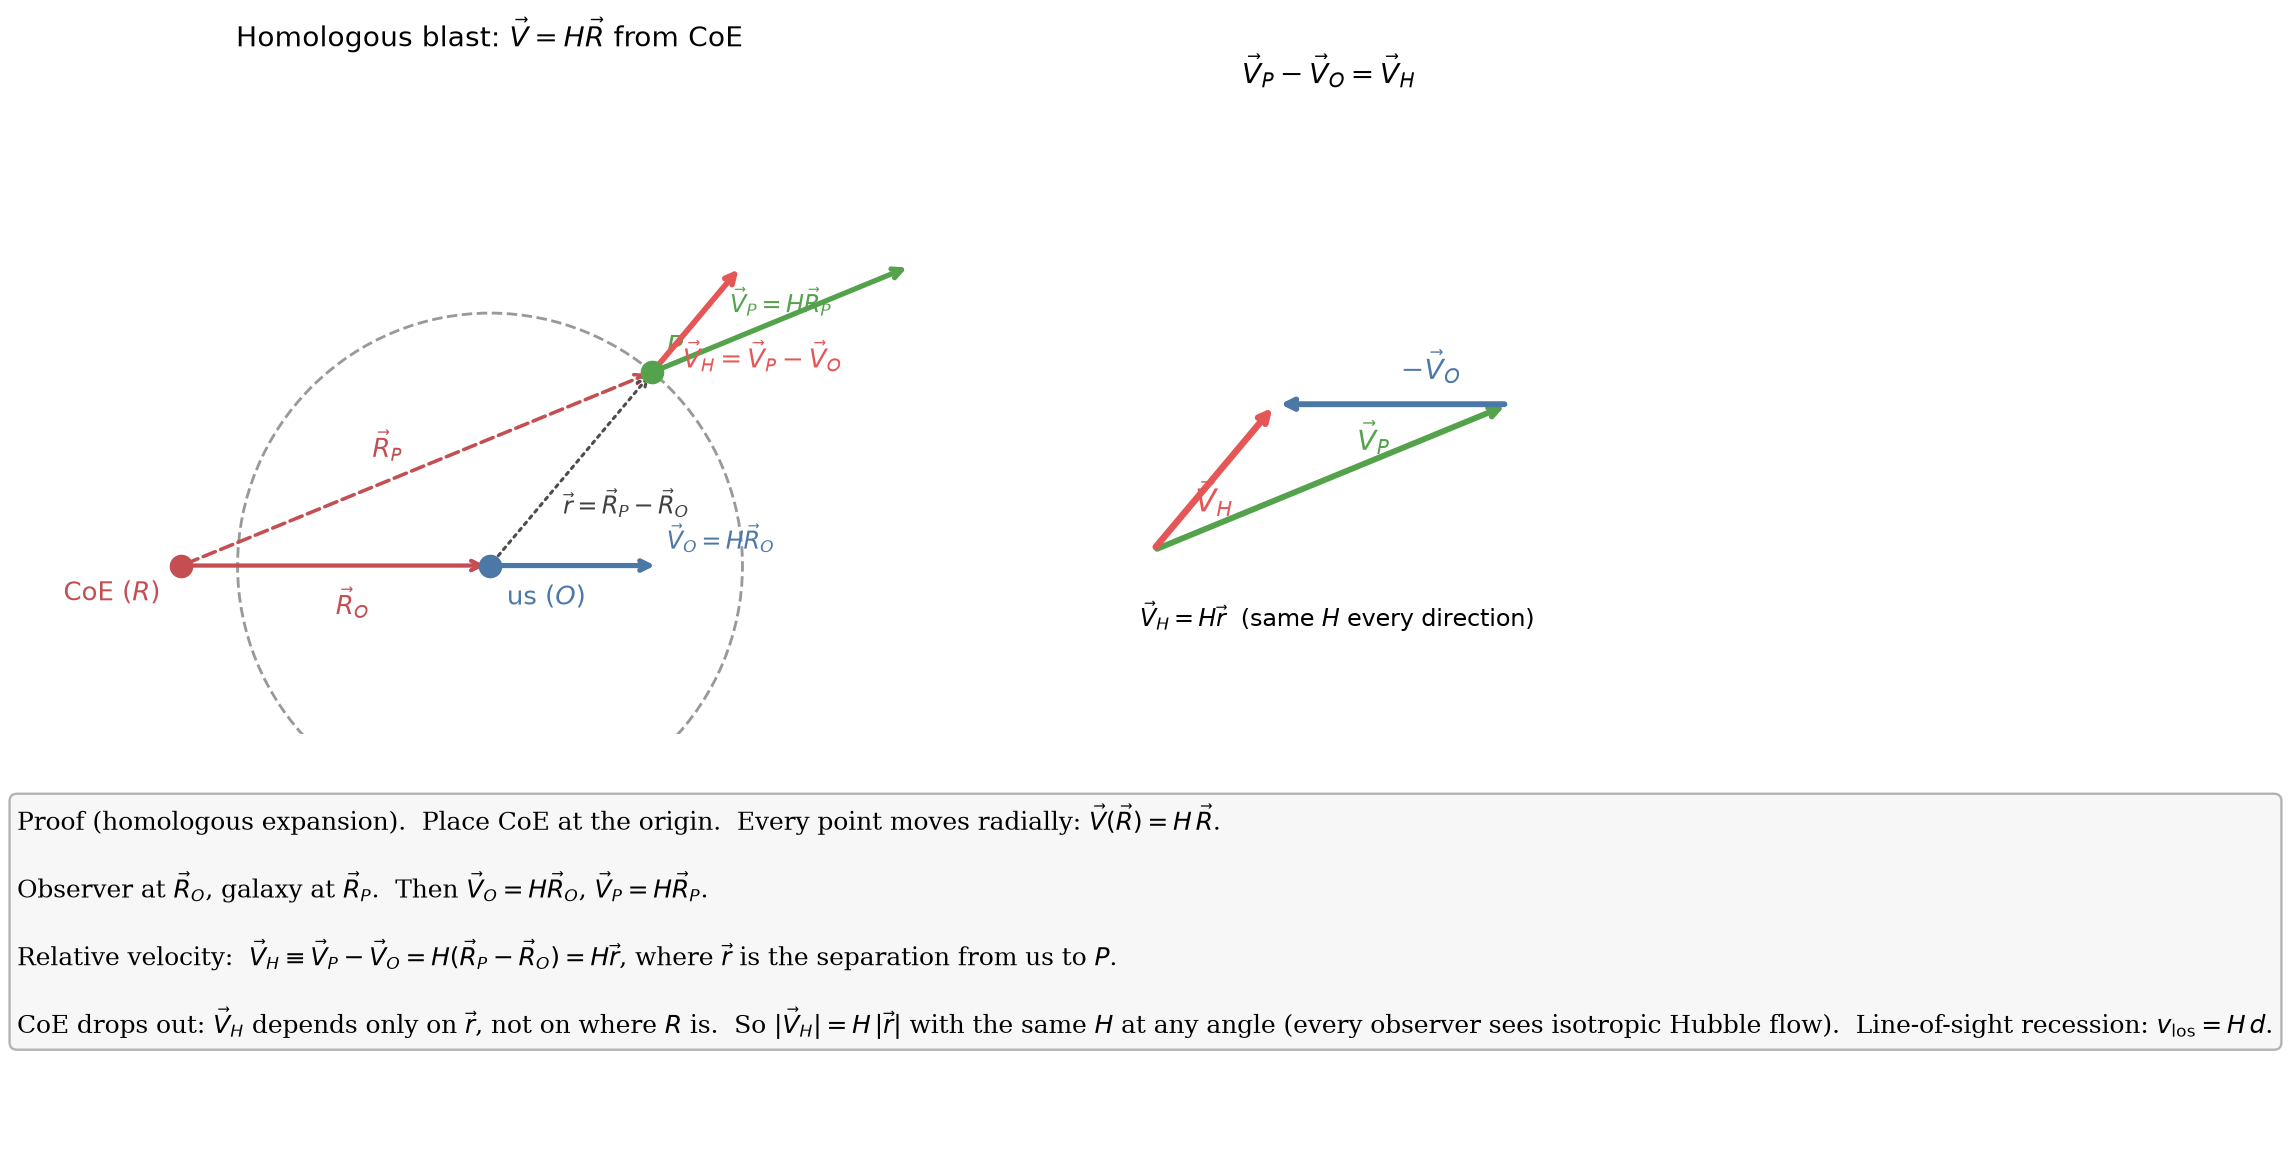
\includegraphics[width=0.90\textwidth]{hubble_from_coe_relative_velocity.png}
\caption{Homologous blast: absolute velocities point away from the CoE, but
$\vec{v}_{\mathrm{rel}}=H\vec{\ell}$ so every observer measures isotropic
$H_{\mathrm{obs}}=H$.}
\label{fig:homology}
\end{figure}

%======================================================================
\section{Decreasing density, enclosed mass, and Gauss $g$}
\label{sec:density}

A uniform ball gives $\vec{g}\propto -\vec{r}$ inside, which preserves
homologous flow and cannot source a sky anisotropy in $H_{\mathrm{obs}}$.
Reject that. Take a spherical, radially decreasing density (toy exponential
used in the journal figure)
\begin{equation}
  \frac{\rho(r)}{\rho_0} = \mathrm{e}^{-r/L},
  \label{eq:rhoexp}
\end{equation}
with scale length $L$. The enclosed-mass fraction with $X\equiv r/L$ is
\begin{equation}
  \frac{m(r)}{M}
  = 1 - \mathrm{e}^{-X}\Bigl(1 + X + \tfrac{1}{2}X^2\Bigr),
  \label{eq:menc}
\end{equation}
which follows by integrating $4\pi r^2\rho(r)$ and normalizing to the total
mass $M$ of the infinite exponential. Gauss / shell theorem then gives
\begin{equation}
  \vec{g}(r) = -\frac{G\,M(<r)}{r^2}\,\hat{r}.
  \label{eq:gauss}
\end{equation}
At the observer distance $D$, a natural dimensionless gravity strength is
\begin{equation}
  \kappa_{\mathrm{natural}}
  = \frac{G\,M_{\mathrm{enc}}(<D)}{D^3 H^2}
  = \frac{\Omega_m}{2}
  = 0.15
  \quad\text{for }\Omega_m=0.3.
  \label{eq:kappa}
\end{equation}
The journal toy panel draws the observer at $D/L=3$ (not the later
recommended-profile $D/L\approx5.9$). Leading multipole of off-center
Gauss+decreasing-$\rho$ is a quadrupole ($P_2$), not a pure dipole---keep
that honest when reading later Amp$\times\sin$ / $2\ell$ templates.

\begin{figure}[ht]
\centering
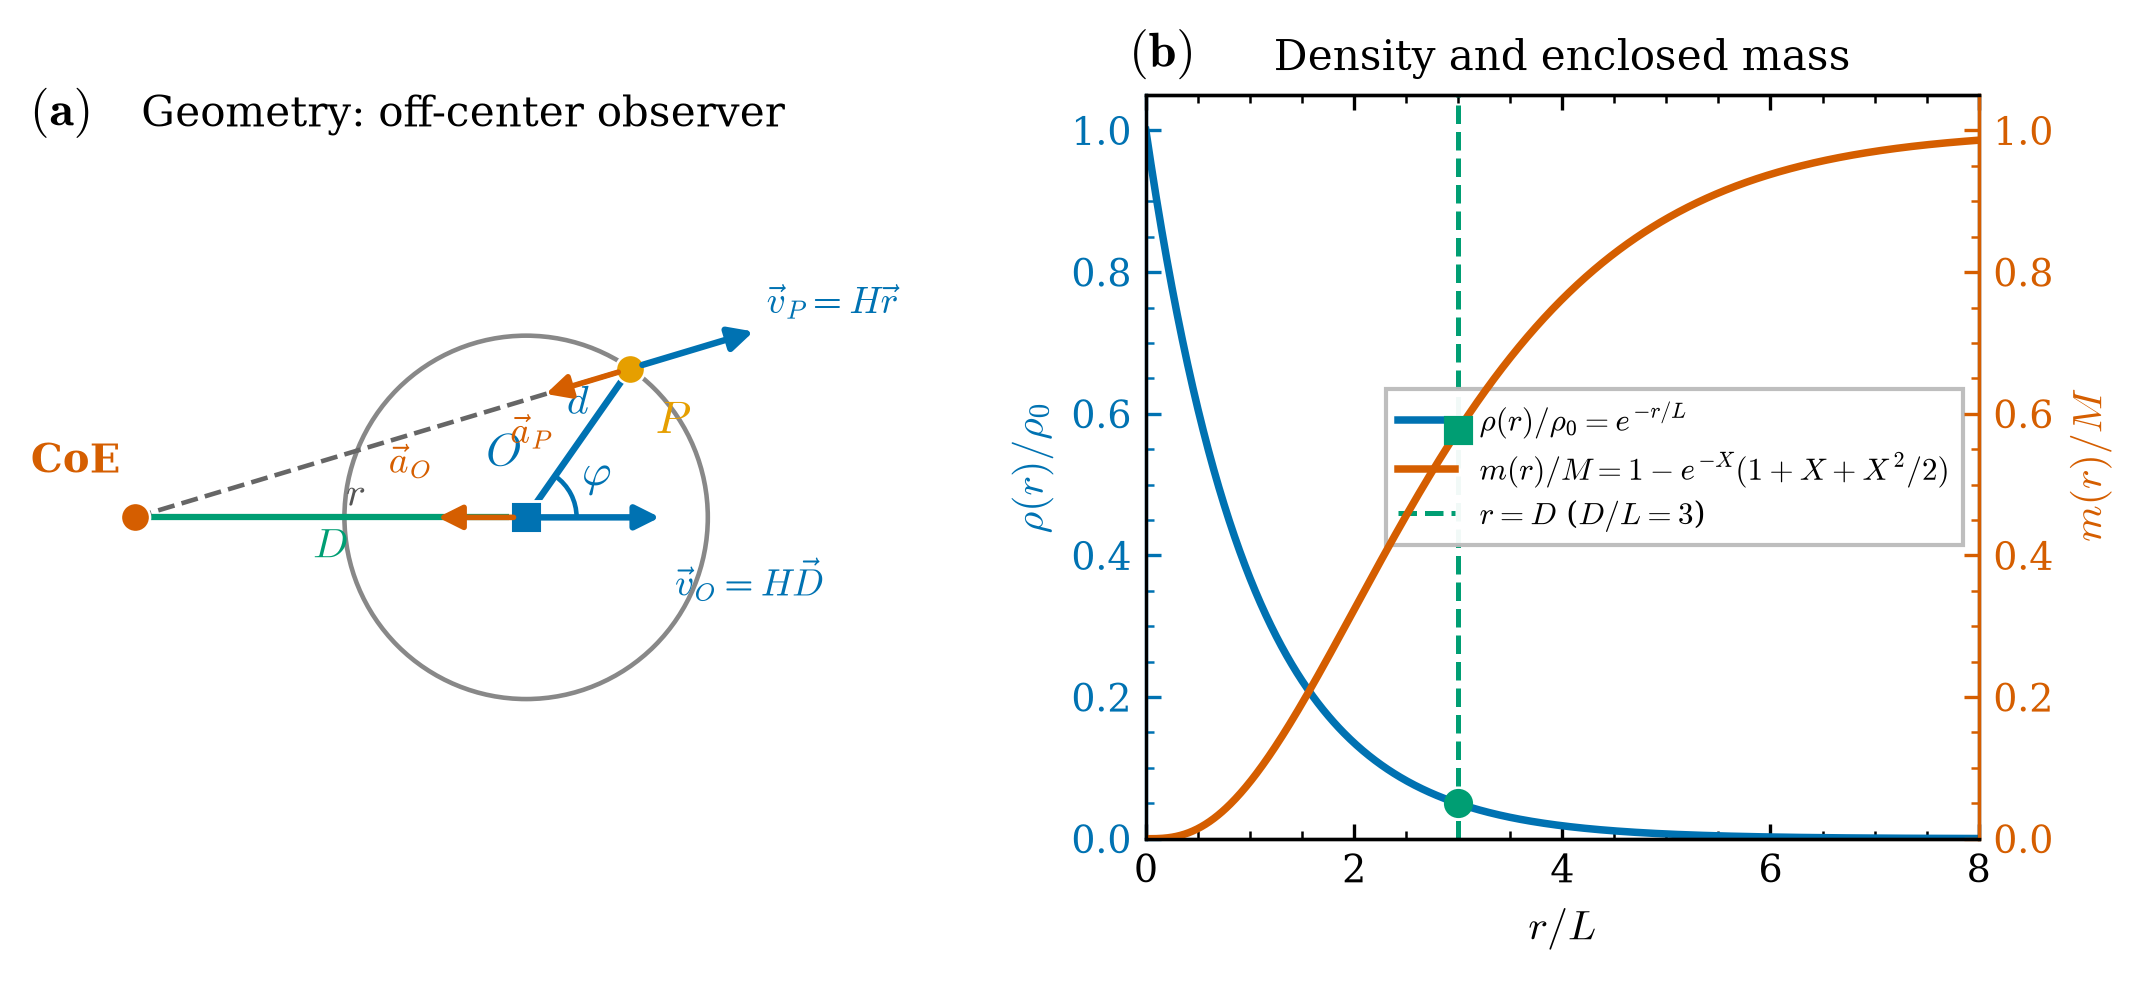
\includegraphics[width=0.92\textwidth]{sedov_decreasing_density_toy_journal.png}
\caption{Toy exponential $\rho(r)/\rho_0=\mathrm{e}^{-r/L}$ and enclosed-mass
fraction $m(r)/M$ from Eq.~\eqref{eq:menc}. Observer mark at $D/L=3$ as in
the journal figure sidecar.}
\label{fig:sedov}
\end{figure}

%======================================================================
\section{Ideal-integration ST+Gauss: $A$ vs angle (sheet AF)}
\label{sec:AF}

Geometry: CoE at the origin, observer at distance $D$, sources sampled at
observer-centric depth $d$, Earth-centric angle measured from the preferred
axis $\hat{D}$. The Migkas $A$ proxy used on the sheet AF series is
\begin{equation}
  A \;\propto\; \frac{H_{\mathrm{obs}}}{H}
  \qquad\text{(sheet AF; mean-renormed on the strip as needed).}
  \label{eq:Aproxy}
\end{equation}
(Alternate cards use an inverse-square luminosity-distance mapping
$A_{\mathrm{raw}}\propto 1/(H_{\mathrm{obs}}/H)^2$; the ideal-integration
panel below is the sheet AF $H$-ratio series.) First-principles ST+Gauss
geometry alone (no Amp$\times\sin$) reaches only $R^2_A\approx0.543$ on the
digitized Migkas Fig.~6 strip (summary CSV:
\texttt{geometry\_or\_AN\_alone}).

\begin{figure}[ht]
\centering
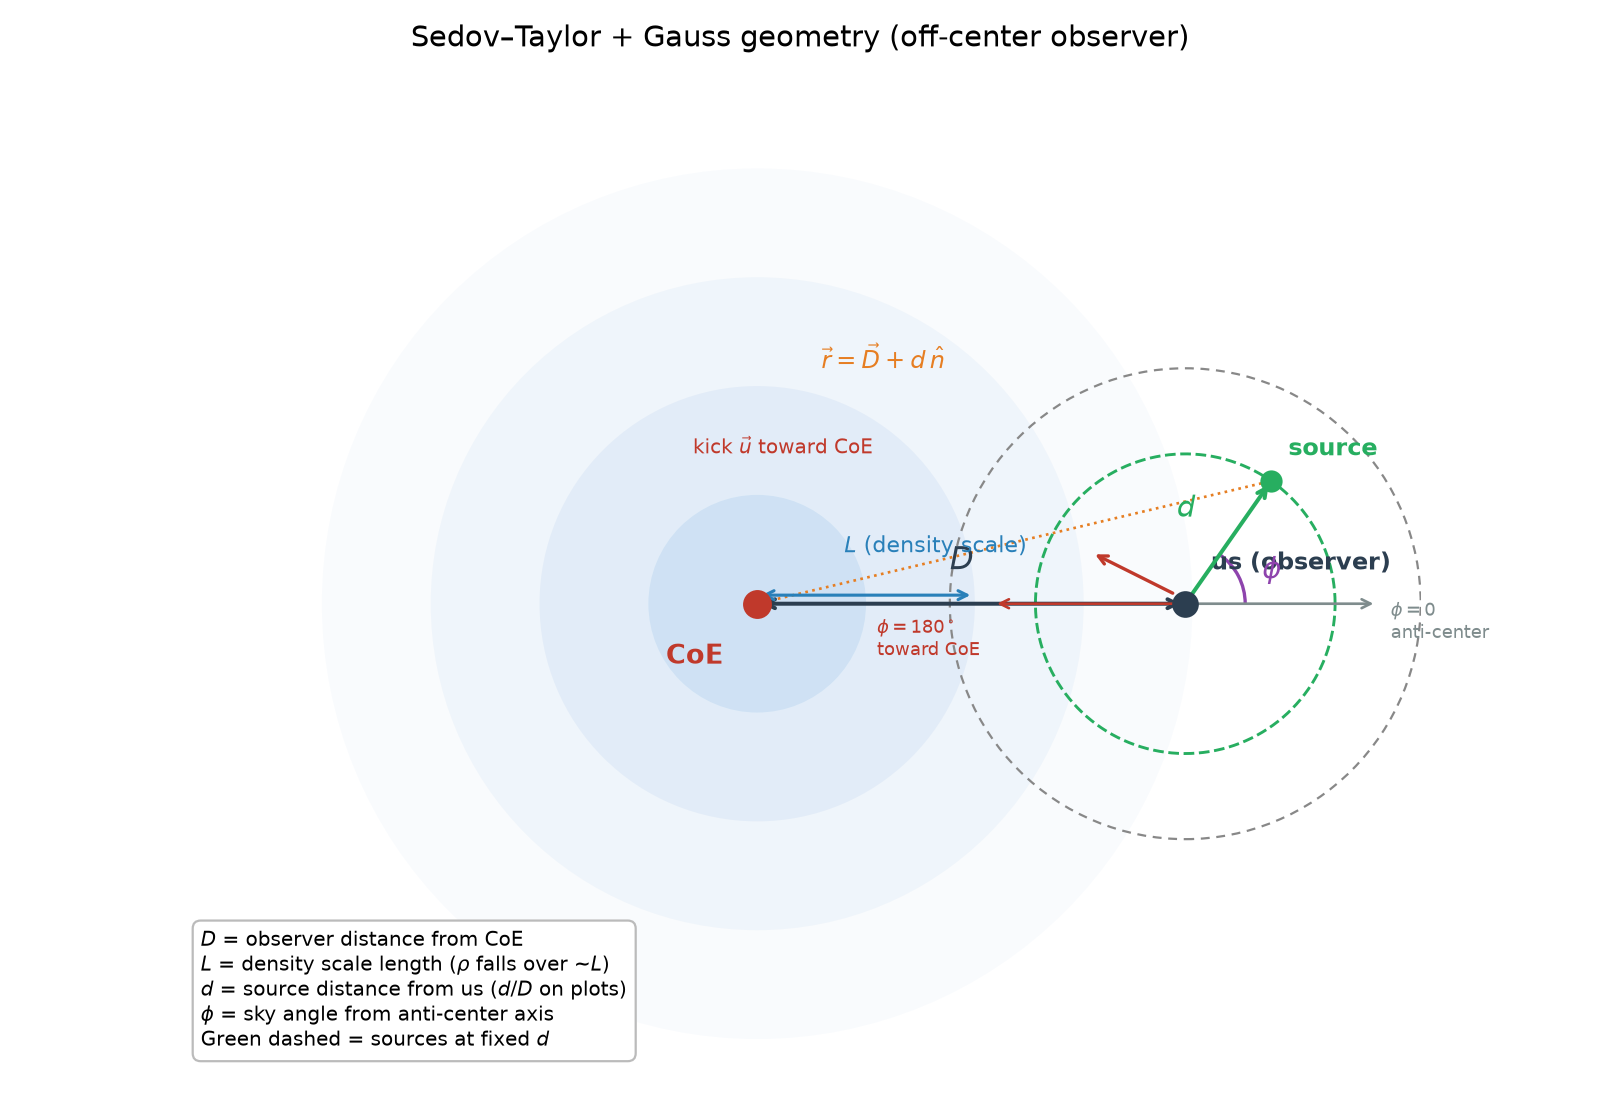
\includegraphics[width=0.72\textwidth]{geometry_CoE_observer.png}
\caption{Optional prior geometry: CoE, observer at $D$, source depth $d$,
angle from the preferred axis.}
\label{fig:geom}
\end{figure}

\begin{figure}[ht]
\centering
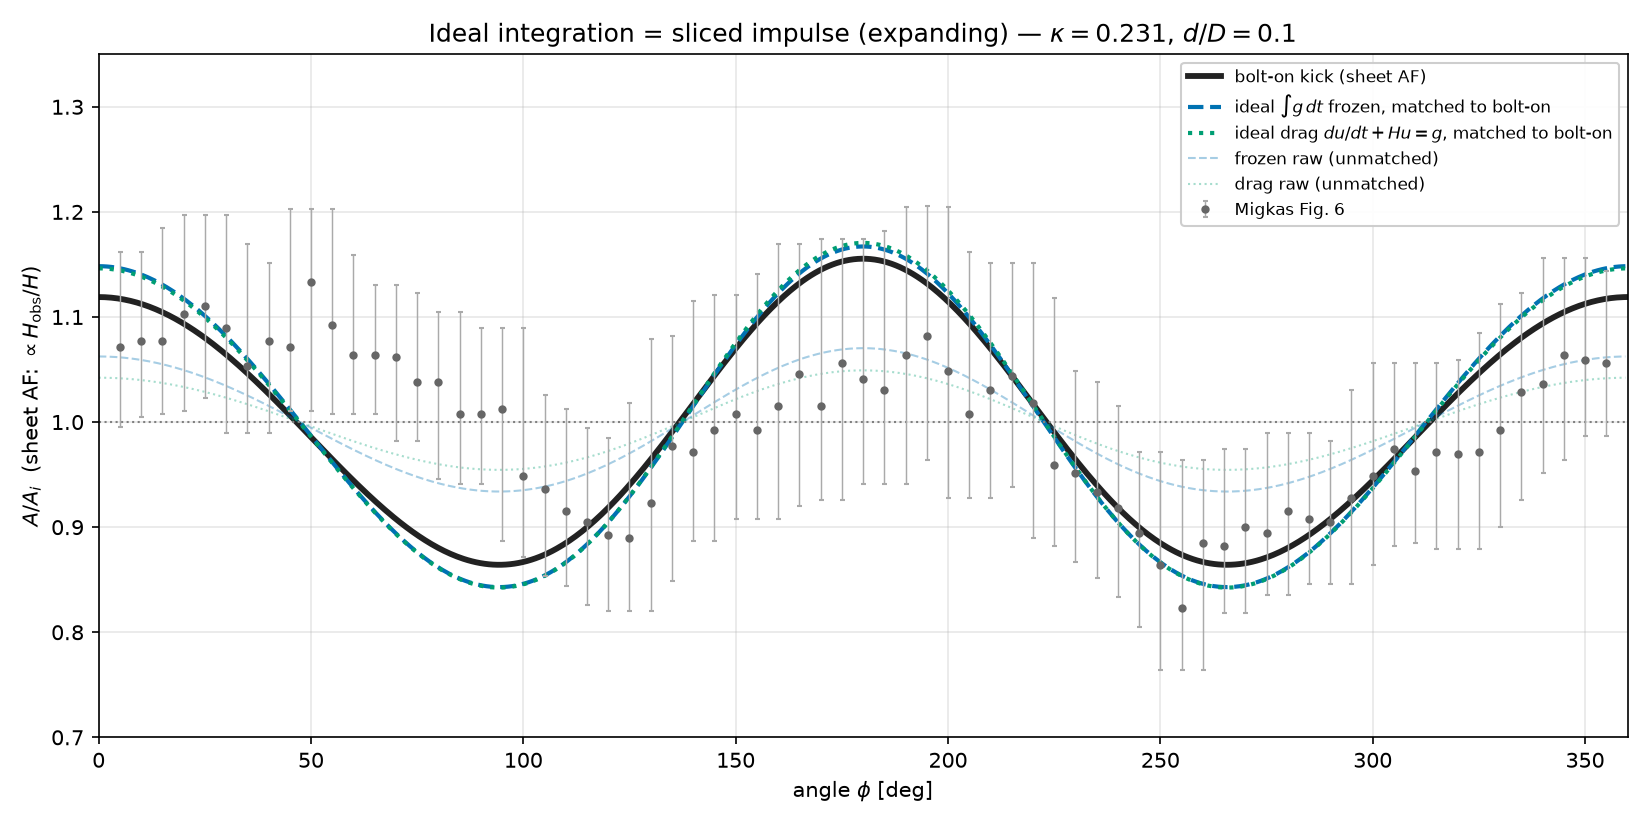
\includegraphics[width=0.92\textwidth]{A_vs_angle_ideal_integration_sheet_AF.png}
\caption{Ideal-integration ST+Gauss $A$ vs Galactic longitude (sheet AF),
before Amp$\times\sin$ or $2\ell$.}
\label{fig:AF}
\end{figure}

%======================================================================
\section{Axisymmetric AF + sine-rotation analogue + residuals}
\label{sec:axisym}

Before the Amp$\times\sin$ template, an axisymmetric rotation analogue
compares AF$_\mathrm{smooth}$ to a rotated smooth curve. On-disk sidecar
\texttt{A\_vs\_angle\_axisymmetric\_before\_rotation\_with\_residuals.json}:
\begin{equation}
  R^2_{\mathrm{before}}\approx0.307,\quad
  \mathrm{RMSE}_{\mathrm{before}}\approx0.059;\qquad
  R^2_{\mathrm{after}}\approx0.553,\quad
  \mathrm{RMSE}_{\mathrm{after}}\approx0.047.
\end{equation}
This panel is \emph{not} Amp$\times\sin$ and \emph{not} $2\ell$; it is the
axisymmetric sine-rotation analogue only.

\begin{figure}[ht]
\centering
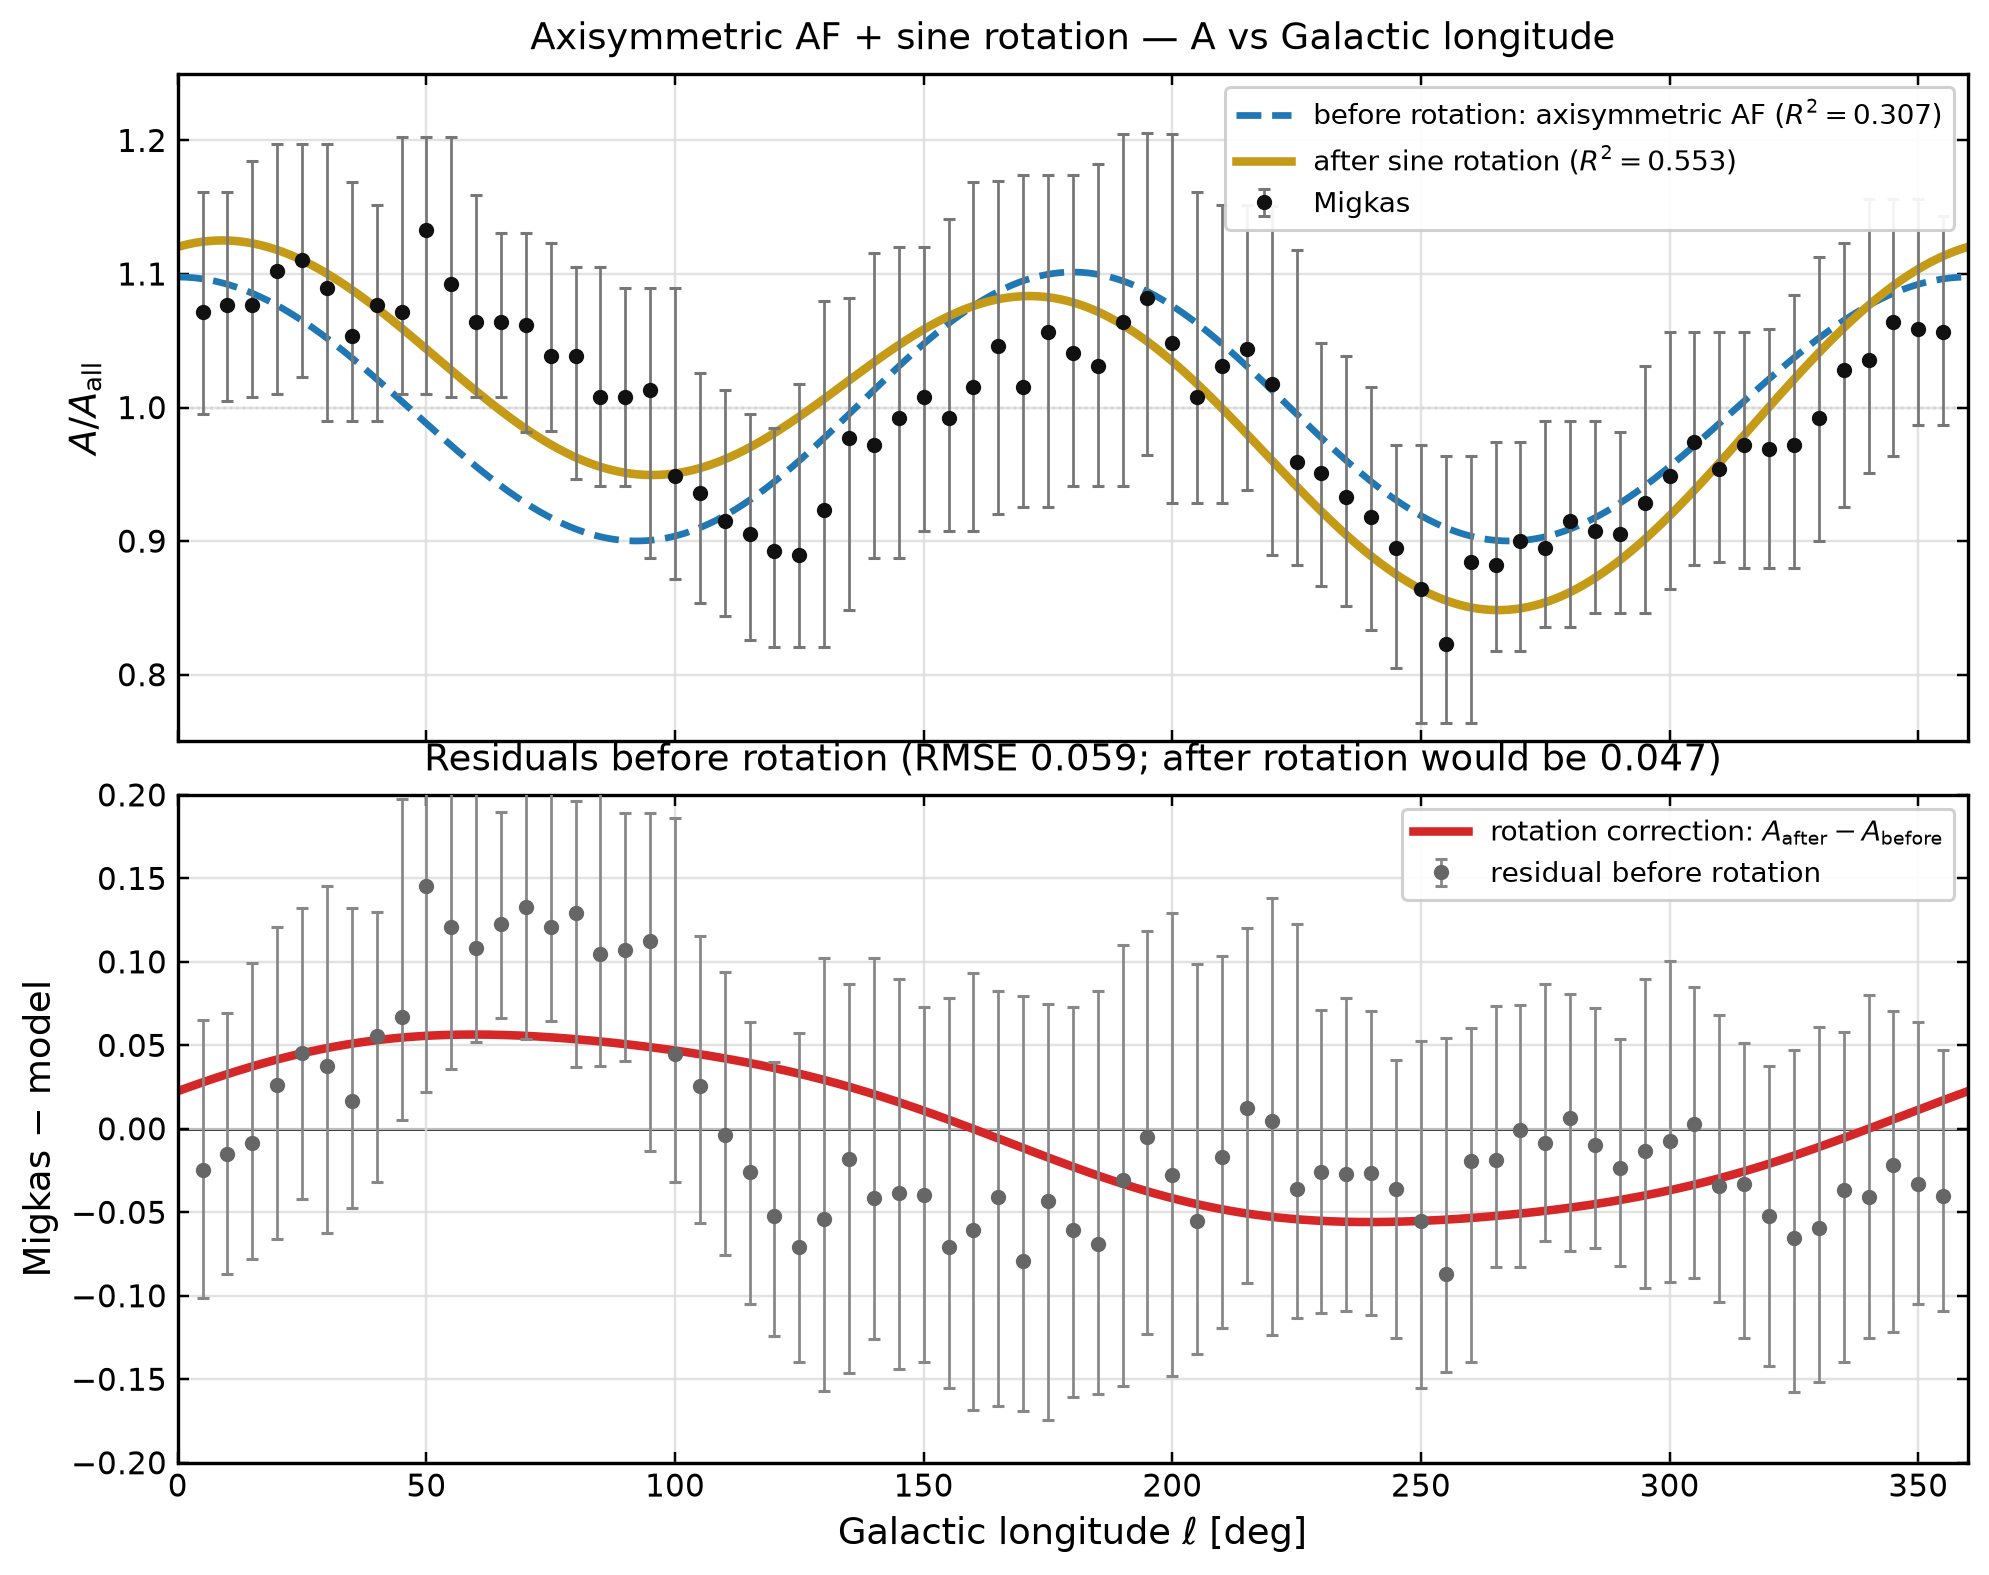
\includegraphics[width=0.92\textwidth]{A_vs_angle_axisymmetric_before_rotation_with_residuals.png}
\caption{Axisymmetric AF before/after sine-rotation analogue, with residuals.
$R^2\approx0.307\to0.553$; RMSE $\approx0.059\to0.047$.}
\label{fig:axisym}
\end{figure}

%======================================================================
\section{Amp$\times\sin$ + multiplicative $2\ell$ correction}
\label{sec:ampsin}

\subsection{Amp$\times\sin$ convention (verified)}
Sheet / level-set / cone-scan convention (not first-principles Gauss):
\begin{equation}
  A'(\ell)
  = \bigl(1 - \mathrm{Amp}_A\cdot\sin(\Omega\ell + \phi)\bigr)\,A_{\mathrm{physics}},
  \qquad
  \Omega = \frac{2\pi}{360},
  \label{eq:ampsin}
\end{equation}
with $\ell$ in degrees and $\phi$ in radians in the same trig argument
(sidecar scripts use $\phi$ in rad). Associated $B$ uses the same sine with
an independent amplitude $\mathrm{Amp}_B$ (shared-opp scans often take
$\mathrm{Amp}_B=-\mathrm{Amp}_A$). Summary CSV peak for $A$:
$\mathrm{Amp}_A=-0.06$, $\phi\approx11.46^\circ$, $R^2_A\approx0.746$.
Shared-opp at that peak: $\mathrm{Amp}_B=+0.06$, $R^2_B\approx0.790$.

\subsection{$2\ell$ multiplier}
Multiplicative residual layer tuned on the Amp$\times\sin$ $A$ curve
(\texttt{best\_fit\_2ell\_multiplier.npz}):
\begin{equation}
  A_{\mathrm{after}}(\ell)
  = \bigl(1 + \varepsilon\cdot\sin(2\ell_{\mathrm{rad}} + \psi)\bigr)
    \,A_{\mathrm{before}}(\ell),
  \label{eq:2ell}
\end{equation}
with $\ell_{\mathrm{rad}}=\ell^\circ\cdot\pi/180$,
$\varepsilon\approx-0.043$, $\psi\approx176^\circ$ (A-tuned).
On disk: $R^2_A\approx0.746\to0.875$; RMSE $\approx0.038\to0.029$.

After-$2\ell$ strip extrema (from $+x$ / anti-CoE in the pose of
Sec.~\ref{sec:rings}): MAX $\approx30^\circ$ and $185^\circ$; MIN $\approx115^\circ$
and $265^\circ$. Highlight bands are
\begin{equation}
  5\%\text{ of }360^\circ = 18^\circ\text{ end-to-end} = \pm9^\circ
  \text{ about each extremum}.
  \label{eq:bands}
\end{equation}

\begin{figure}[ht]
\centering
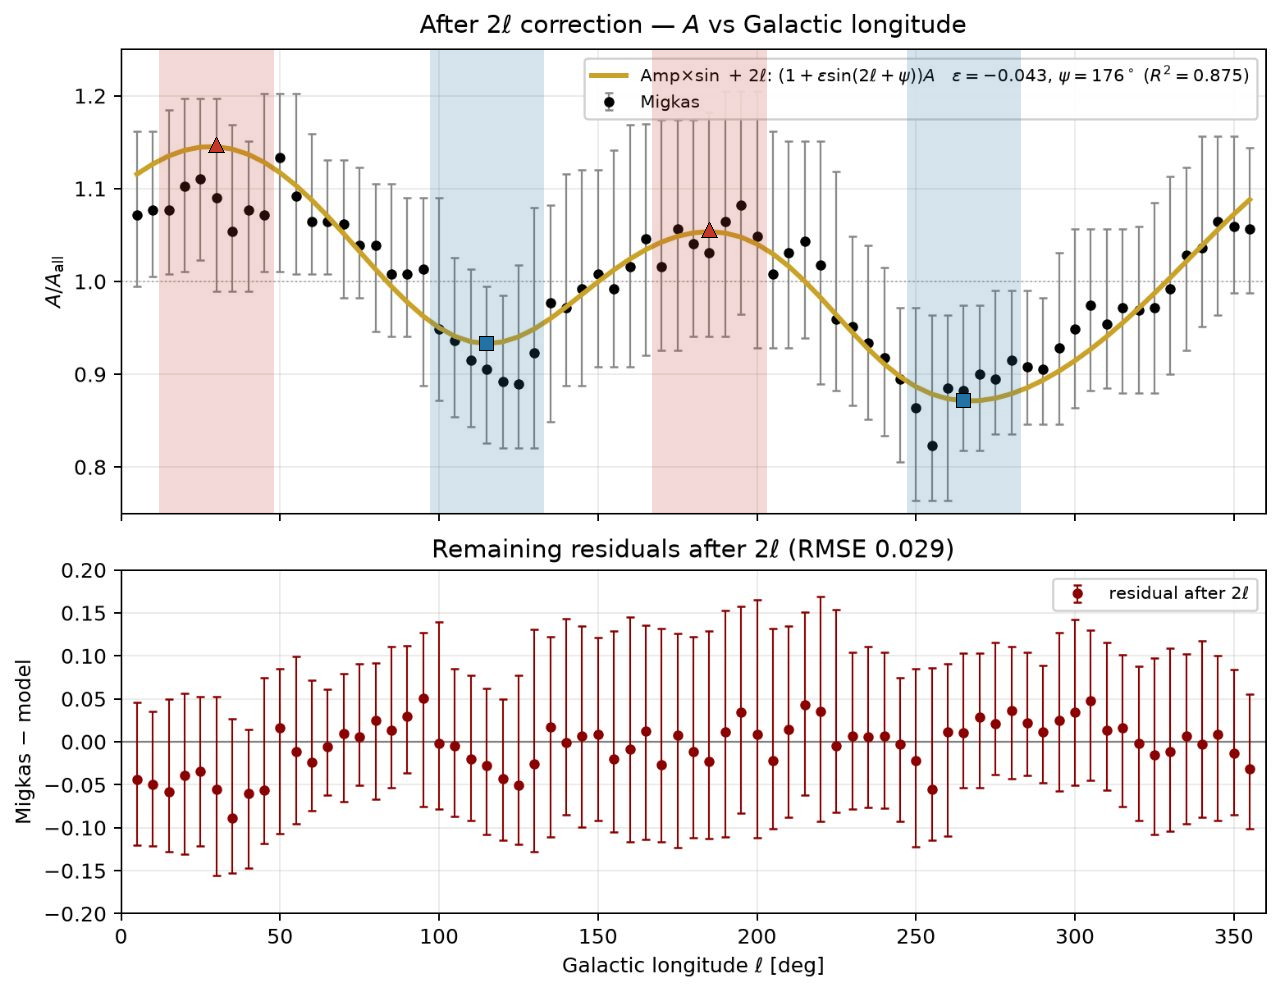
\includegraphics[width=0.92\textwidth]{A_vs_angle_after_2ell_with_residuals.png}
\caption{Amp$\times\sin$ $A(\ell)$ after the $2\ell$ multiplier, with
residuals. Extrema near $30^\circ/185^\circ$ (MAX) and $115^\circ/265^\circ$ (MIN);
bands $\pm9^\circ$ ($18^\circ$ end-to-end). Fit template---not yet derived from
time-integrated gravity.}
\label{fig:2ell}
\end{figure}

%======================================================================
\section{Three-panel CoE rings (2 MAX + 2 MIN)}
\label{sec:rings}

Pose for this draft: anti-CoE at $(\ell,b)=(0^\circ,0^\circ)$, CoE at
$(180^\circ,0^\circ)$; Mollweide with $\ell$ increasing LEFT
($\mathrm{lon}_{\mathrm{disp}}=-\ell_{\mathrm{wrapped}}$). Rings are small
circles of constant $\mu=\hat{n}\cdot\hat{x}$ at the four after-$2\ell$
strip stops, each drawn as one $18^\circ$ end-to-end highlight ($\pm9^\circ$)
plus a mid-stroke.

Real Migkas $A$-map extrema: max $(17^\circ,-9^\circ)$, min $(274^\circ,-22^\circ)$.
Honest note: $(185^\circ,0^\circ)$ and $(115^\circ,0^\circ)$ were strip stand-ins
if still drawn on the three-panel figure.

\begin{figure}[ht]
\centering
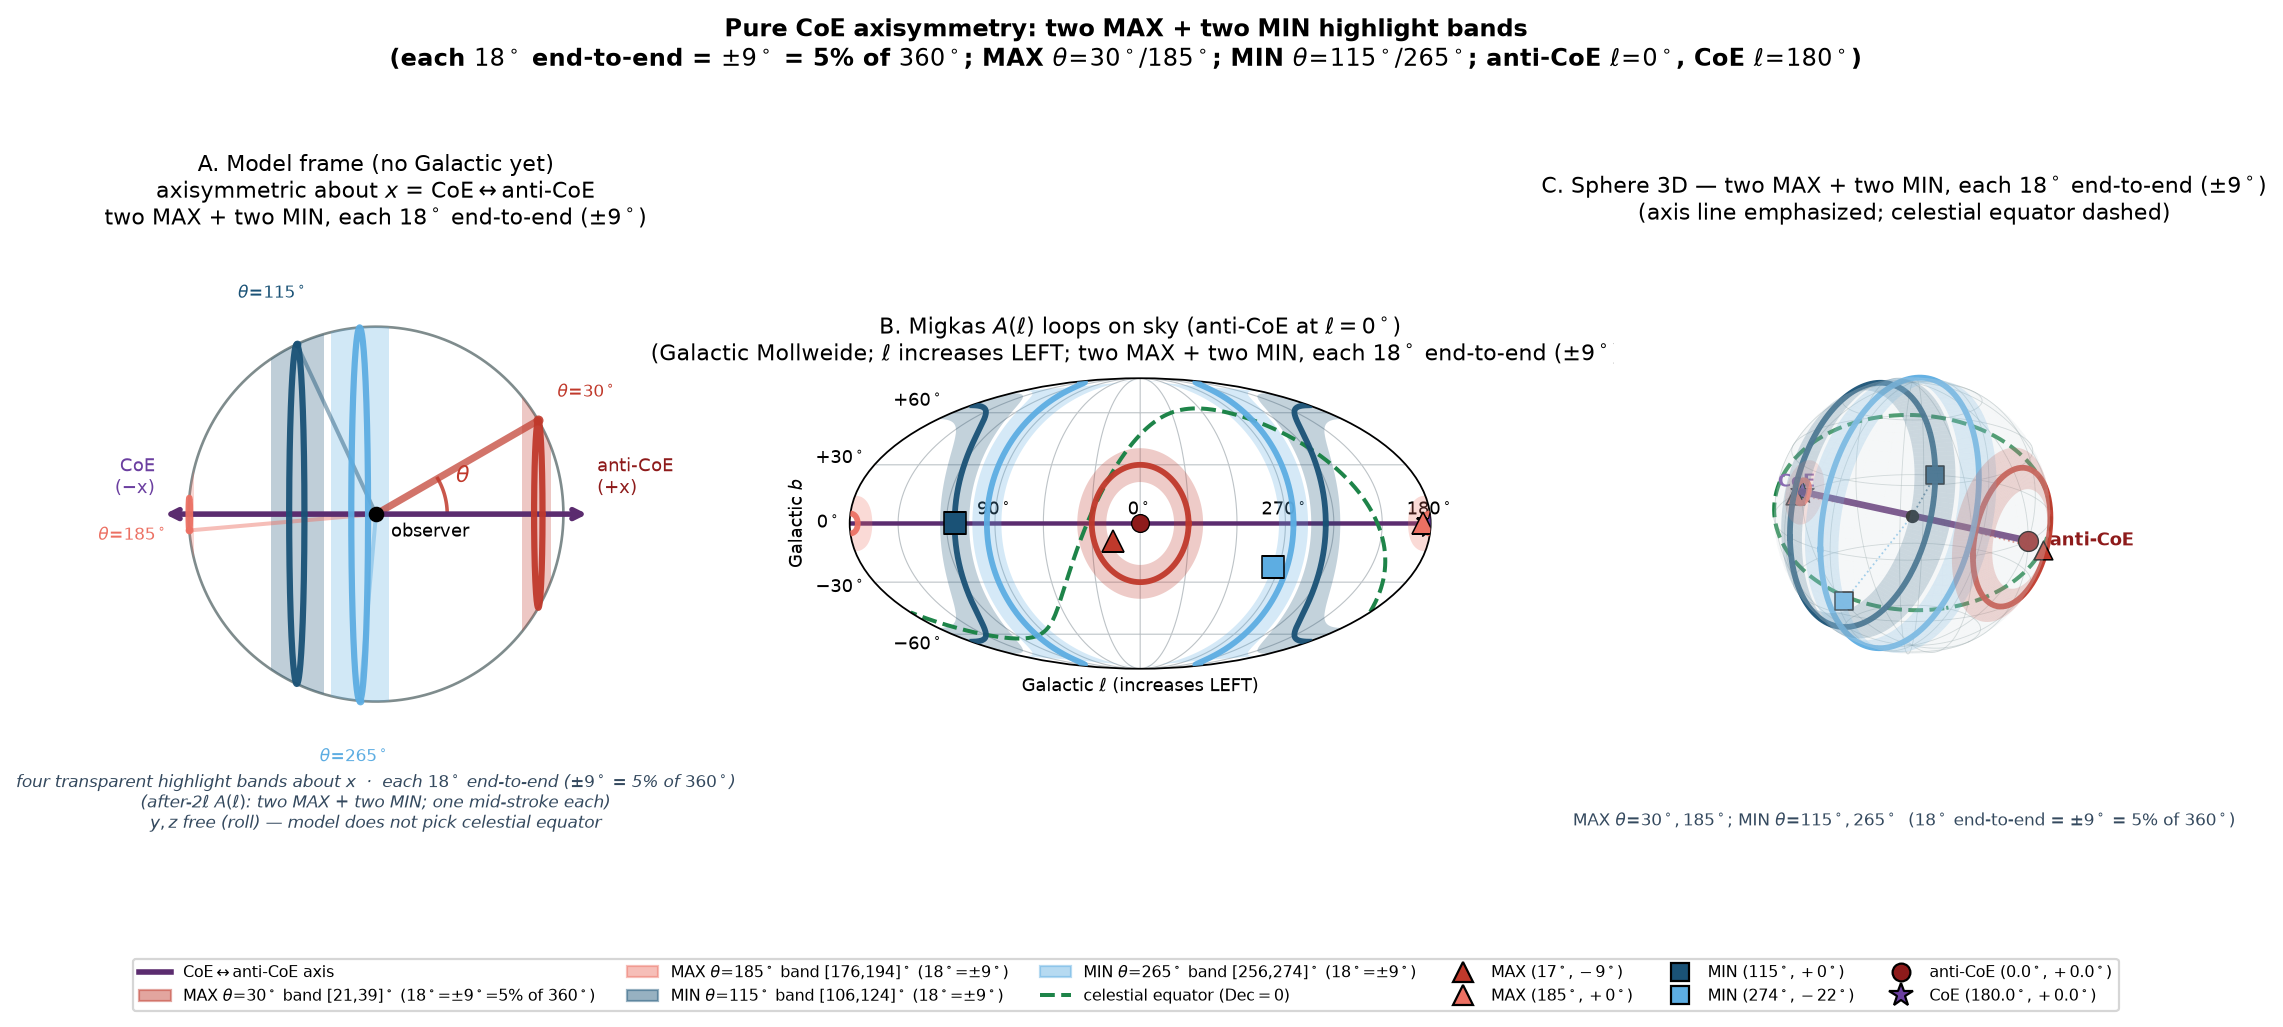
\includegraphics[width=0.98\textwidth]{coe_rings_migkas_pin_axis.png}
\caption{Three-panel CoE rings: strip stops, Mollweide, and sphere. Pose
anti-CoE $(0,0)$ / CoE $(180,0)$. Real Migkas extrema
$(17,-9)$ / $(274,-22)$; strip stand-ins $(185,0)$ / $(115,0)$ if present.}
\label{fig:rings}
\end{figure}

%======================================================================
\section{Migkas Fig.~8 $\theta=75^\circ$ overlay}
\label{sec:migkas8}

Migkas et~al.\ (2020) Fig.~8 ($\theta=75^\circ$ cone $A$ map): lowest $A$ near
$(274^\circ,-22^\circ)$, highest $A$ near $(17^\circ,-9^\circ)$; published dipole
center $(263^\circ,-21^\circ)$ at $3.22\sigma$. Overlay: same four CoE rings /
bands as Sec.~\ref{sec:rings}. $B$ has no published 2D map extrema (slope
flat; fixed to Ball in the Fig.~6 strip analysis).

\begin{figure}[ht]
\centering
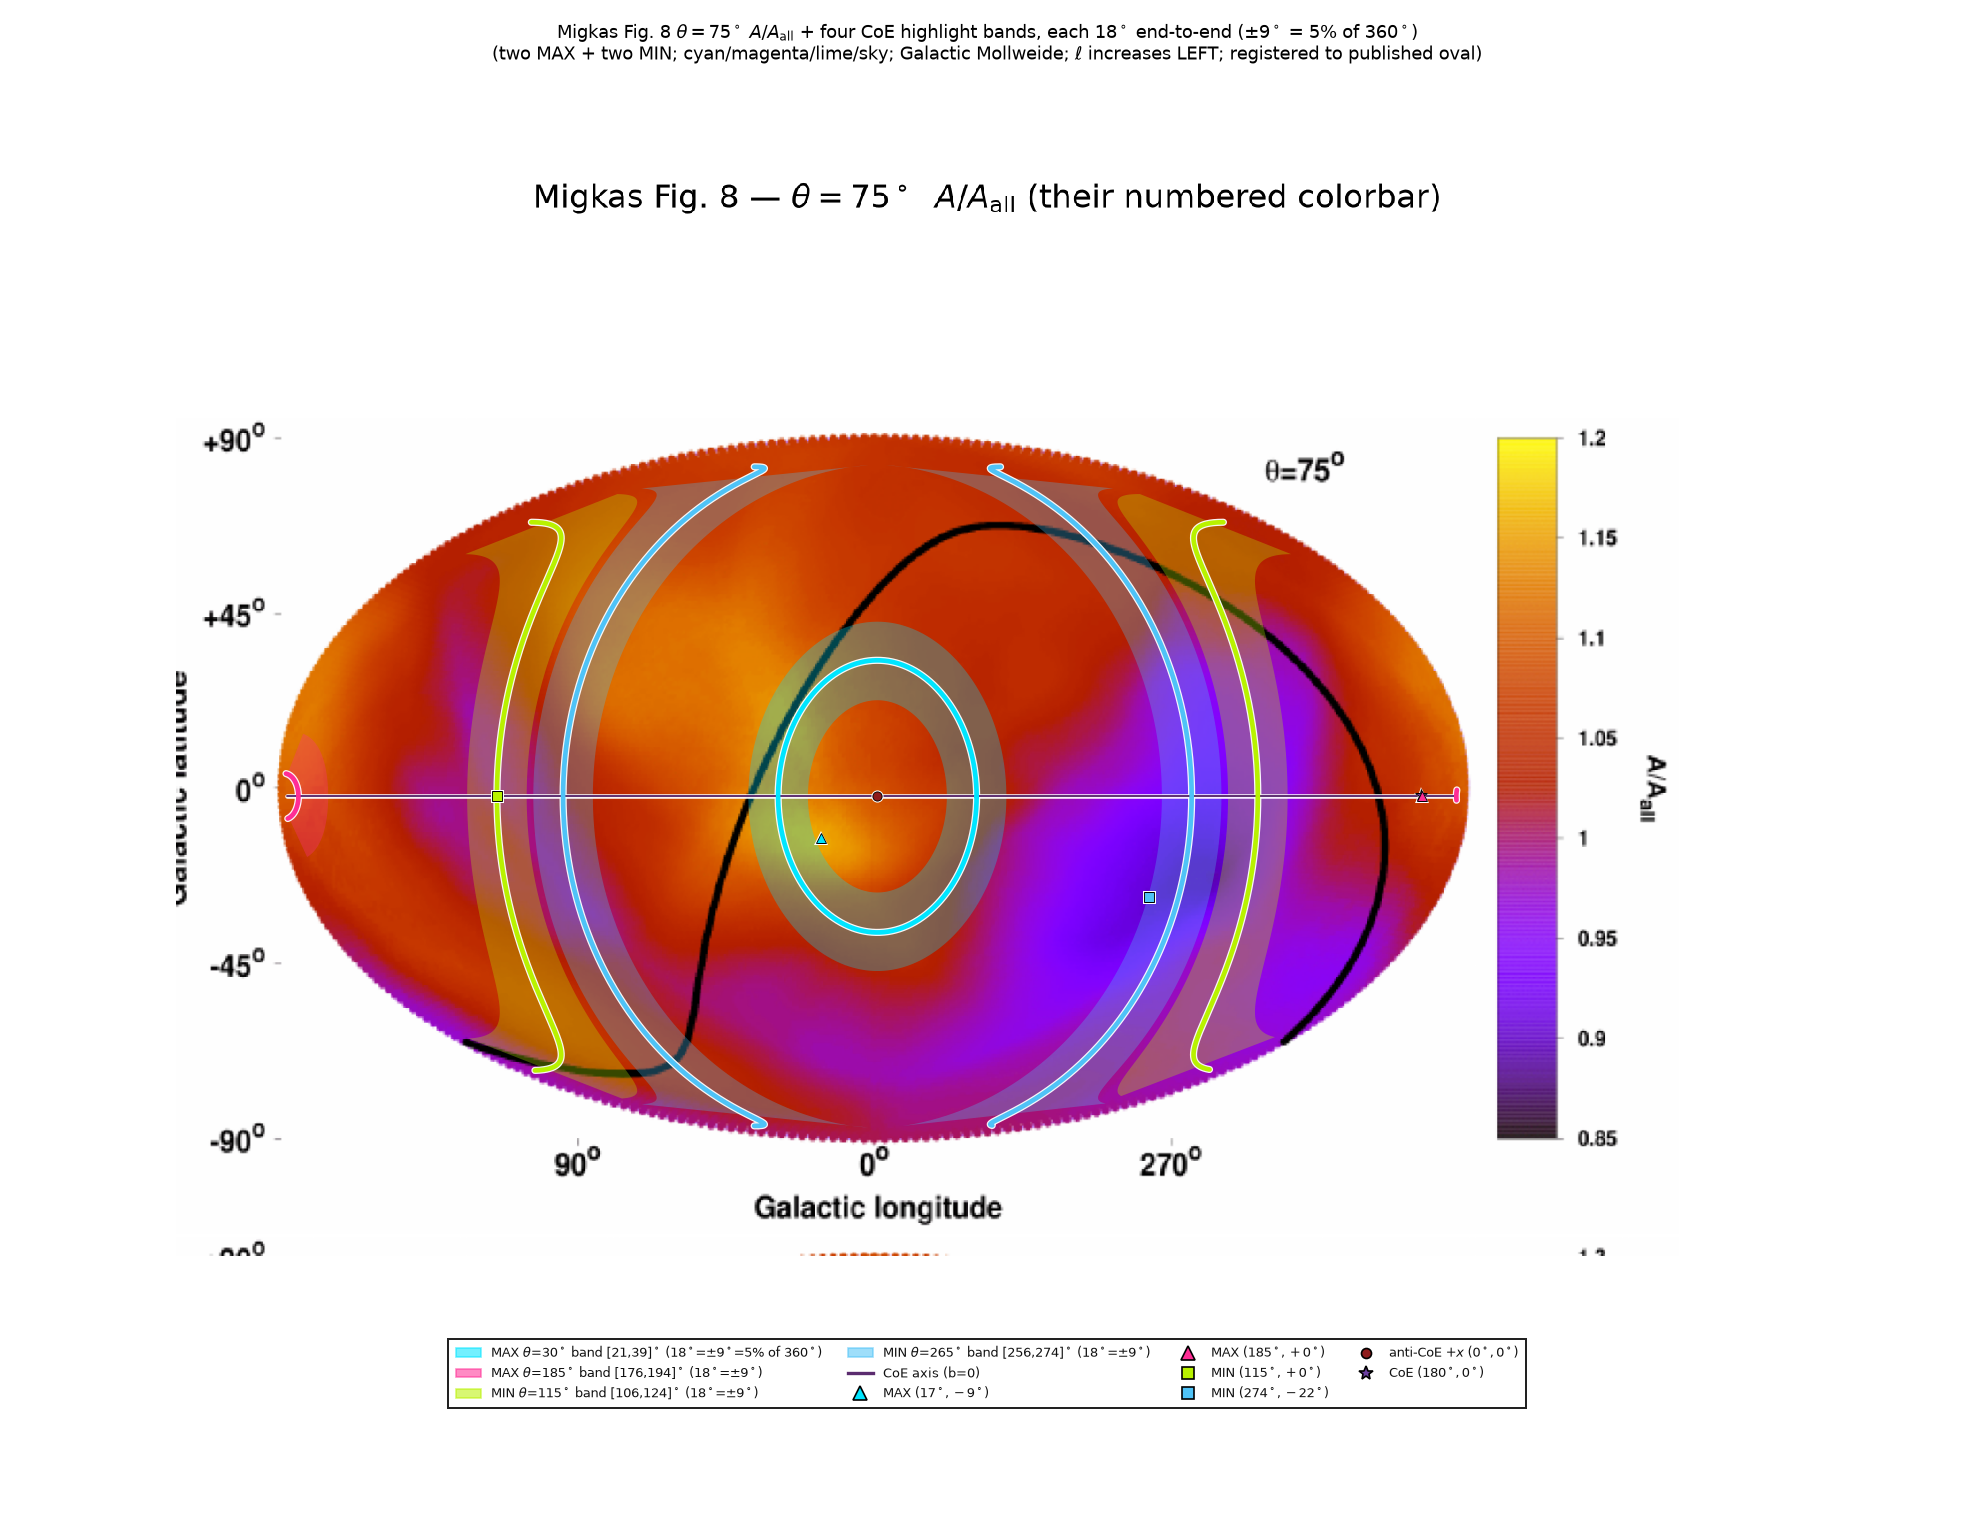
\includegraphics[width=0.98\textwidth]{migkas_fig8_theta75_with_coe_rings.png}
\caption{Migkas Fig.~8 $\theta=75^\circ$ with CoE-ring overlay. Max $A$
$(17,-9)$, min $A$ $(274,-22)$; dipole center $(263,-21)$ at $3.22\sigma$.}
\label{fig:migkas8}
\end{figure}

%======================================================================
\section{Amp/$\phi$ level-set families and $R^2$ heatmaps}
\label{sec:levelsets}

Amp$\times\sin$ is scanned in $(\mathrm{Amp},\phi)$ for $A$ and $B$.
Level-set families and heatmaps below are diagnostics: they map template
depth/phase, not a derived multipole from Gauss.

\begin{figure}[ht]
\centering
\begin{subfigure}[t]{0.48\textwidth}
  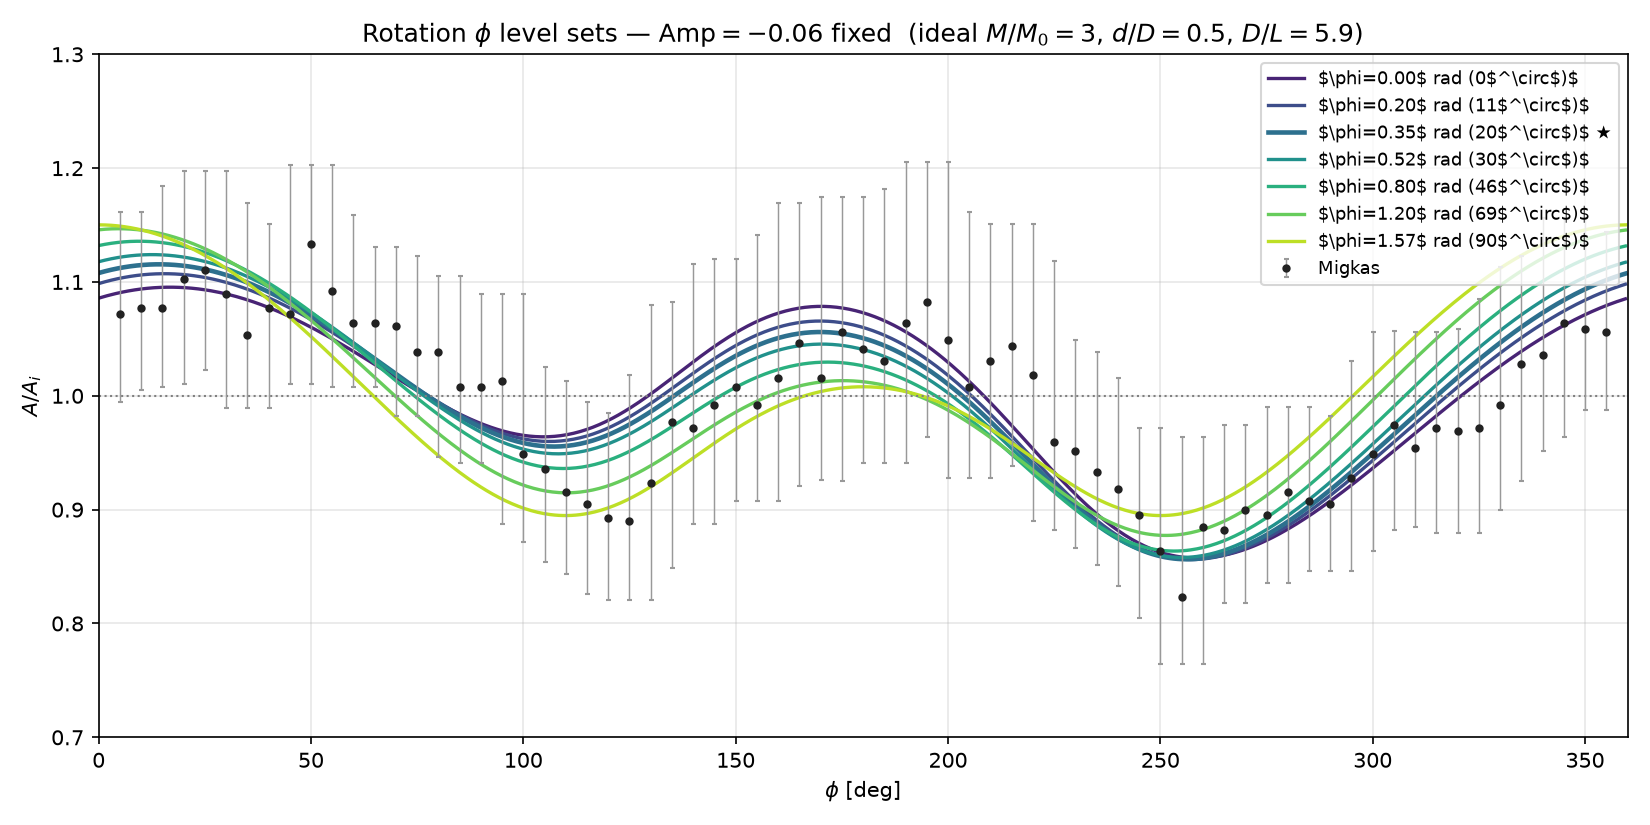
\includegraphics[width=\linewidth]{rotation_levelsets_phi.png}
  \caption{$\phi$ level sets.}
\end{subfigure}\hfill
\begin{subfigure}[t]{0.48\textwidth}
  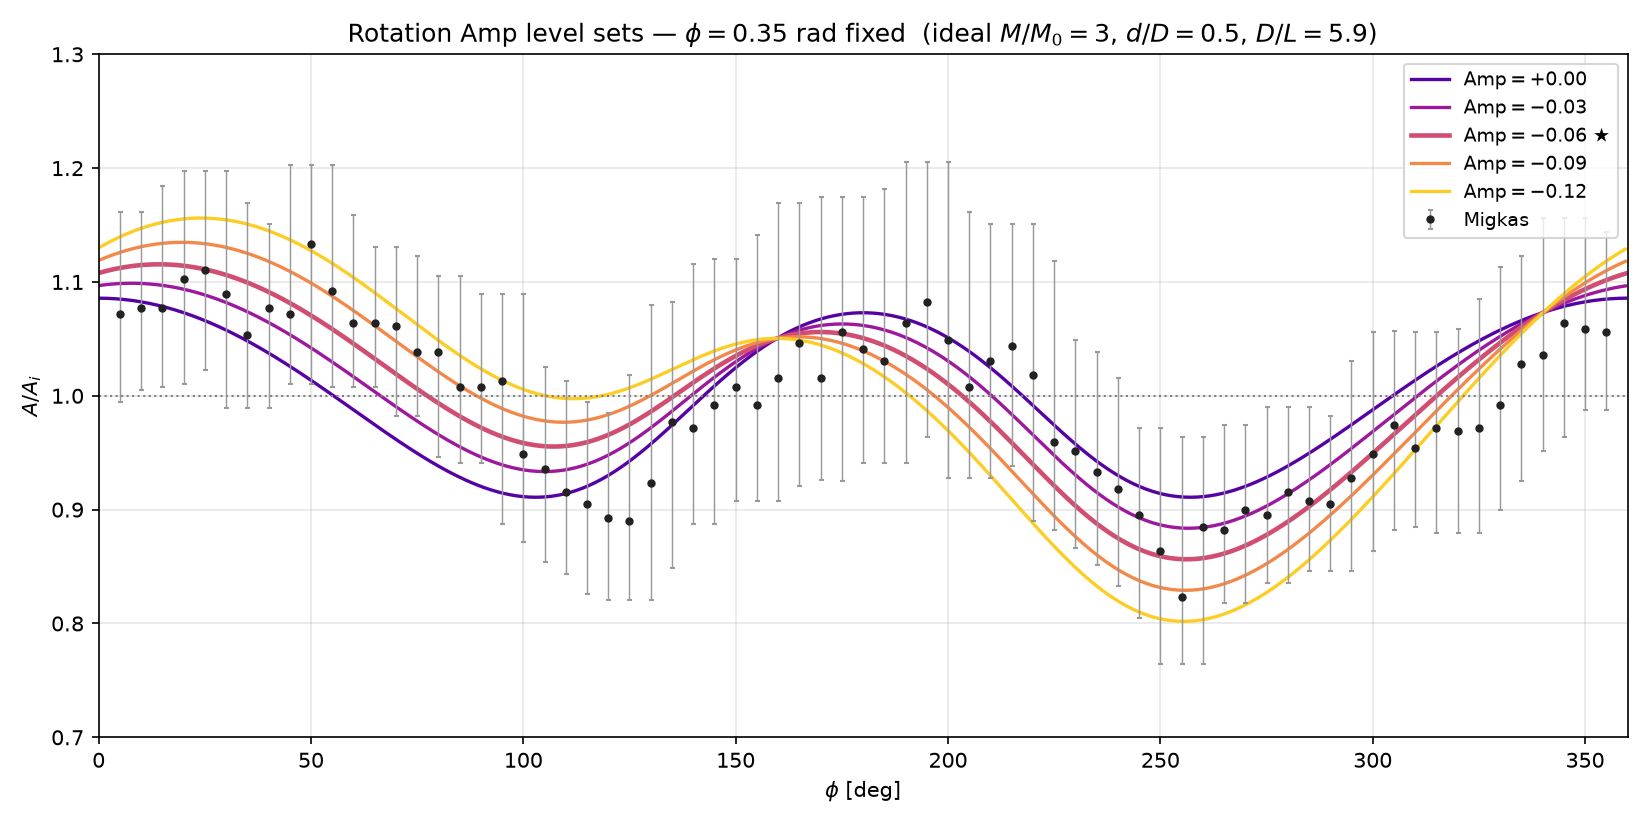
\includegraphics[width=\linewidth]{rotation_levelsets_Amp.png}
  \caption{Amp level sets.}
\end{subfigure}
\caption{Rotation level-set families in $\phi$ and Amp.}
\label{fig:levelsets}
\end{figure}

\begin{figure}[ht]
\centering
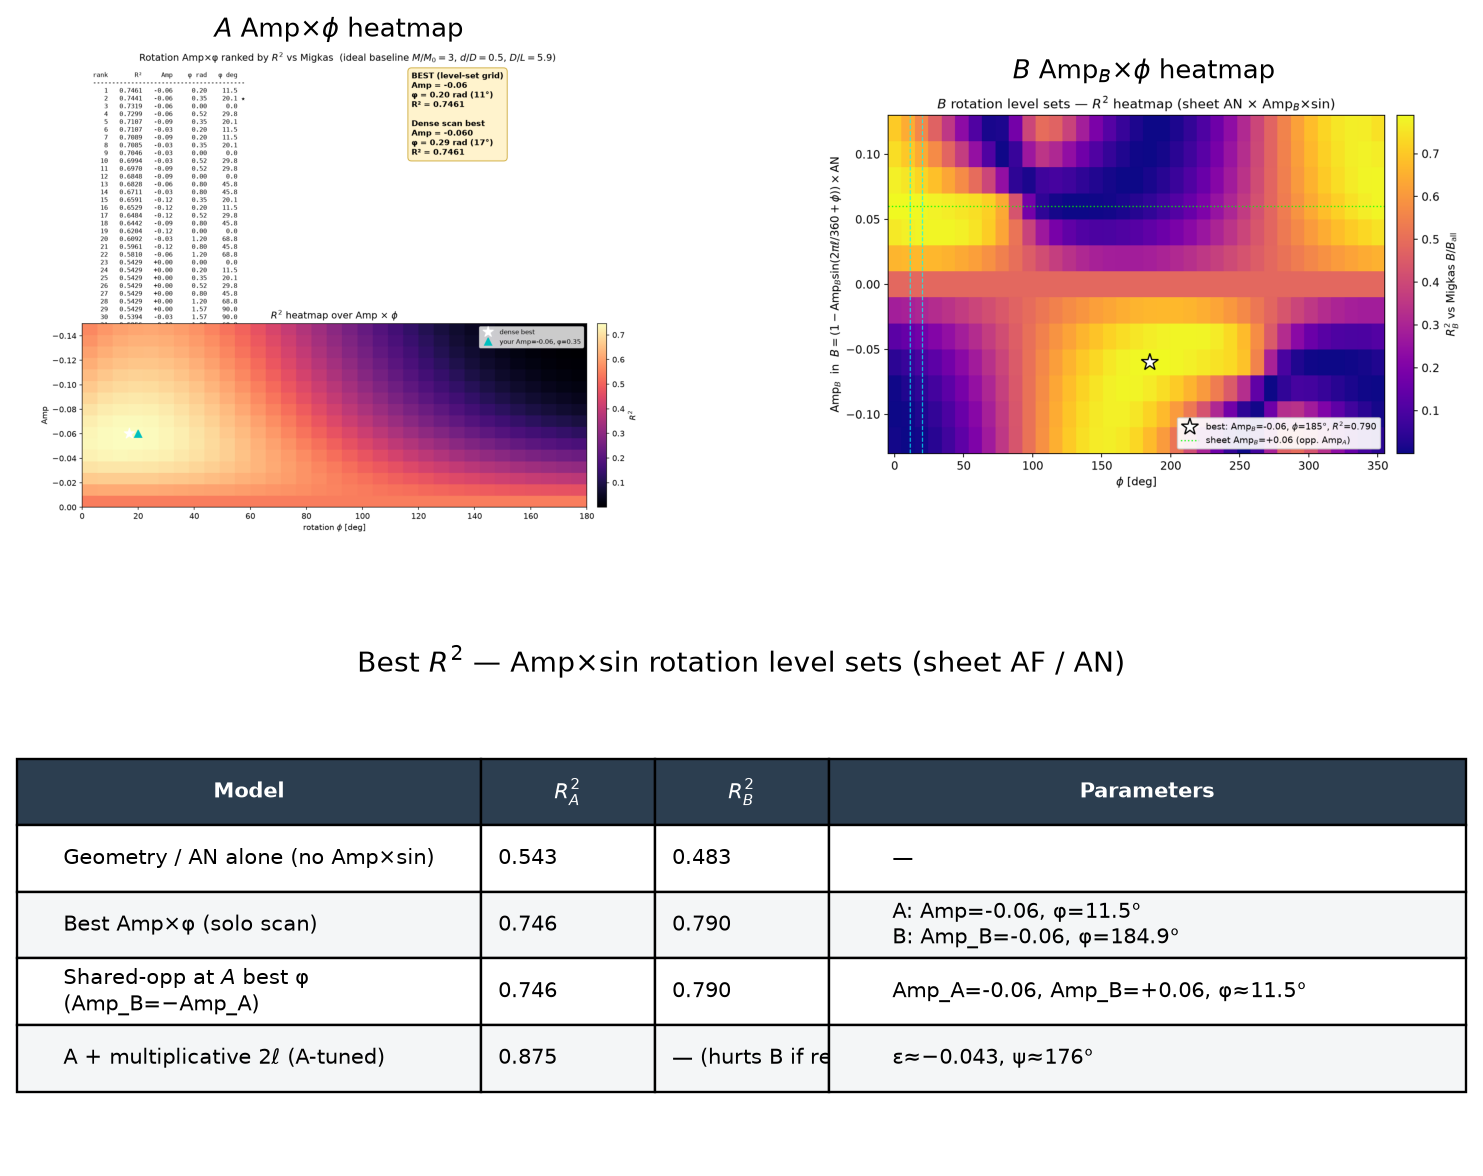
\includegraphics[width=0.95\textwidth]{R2_table_best_A_B_with_heatmaps.png}
\caption{$R^2$ table and heatmaps for best $A$/$B$ Amp$\times\phi$ scans
(summary CSV companion).}
\label{fig:r2table}
\end{figure}

\begin{figure}[ht]
\centering
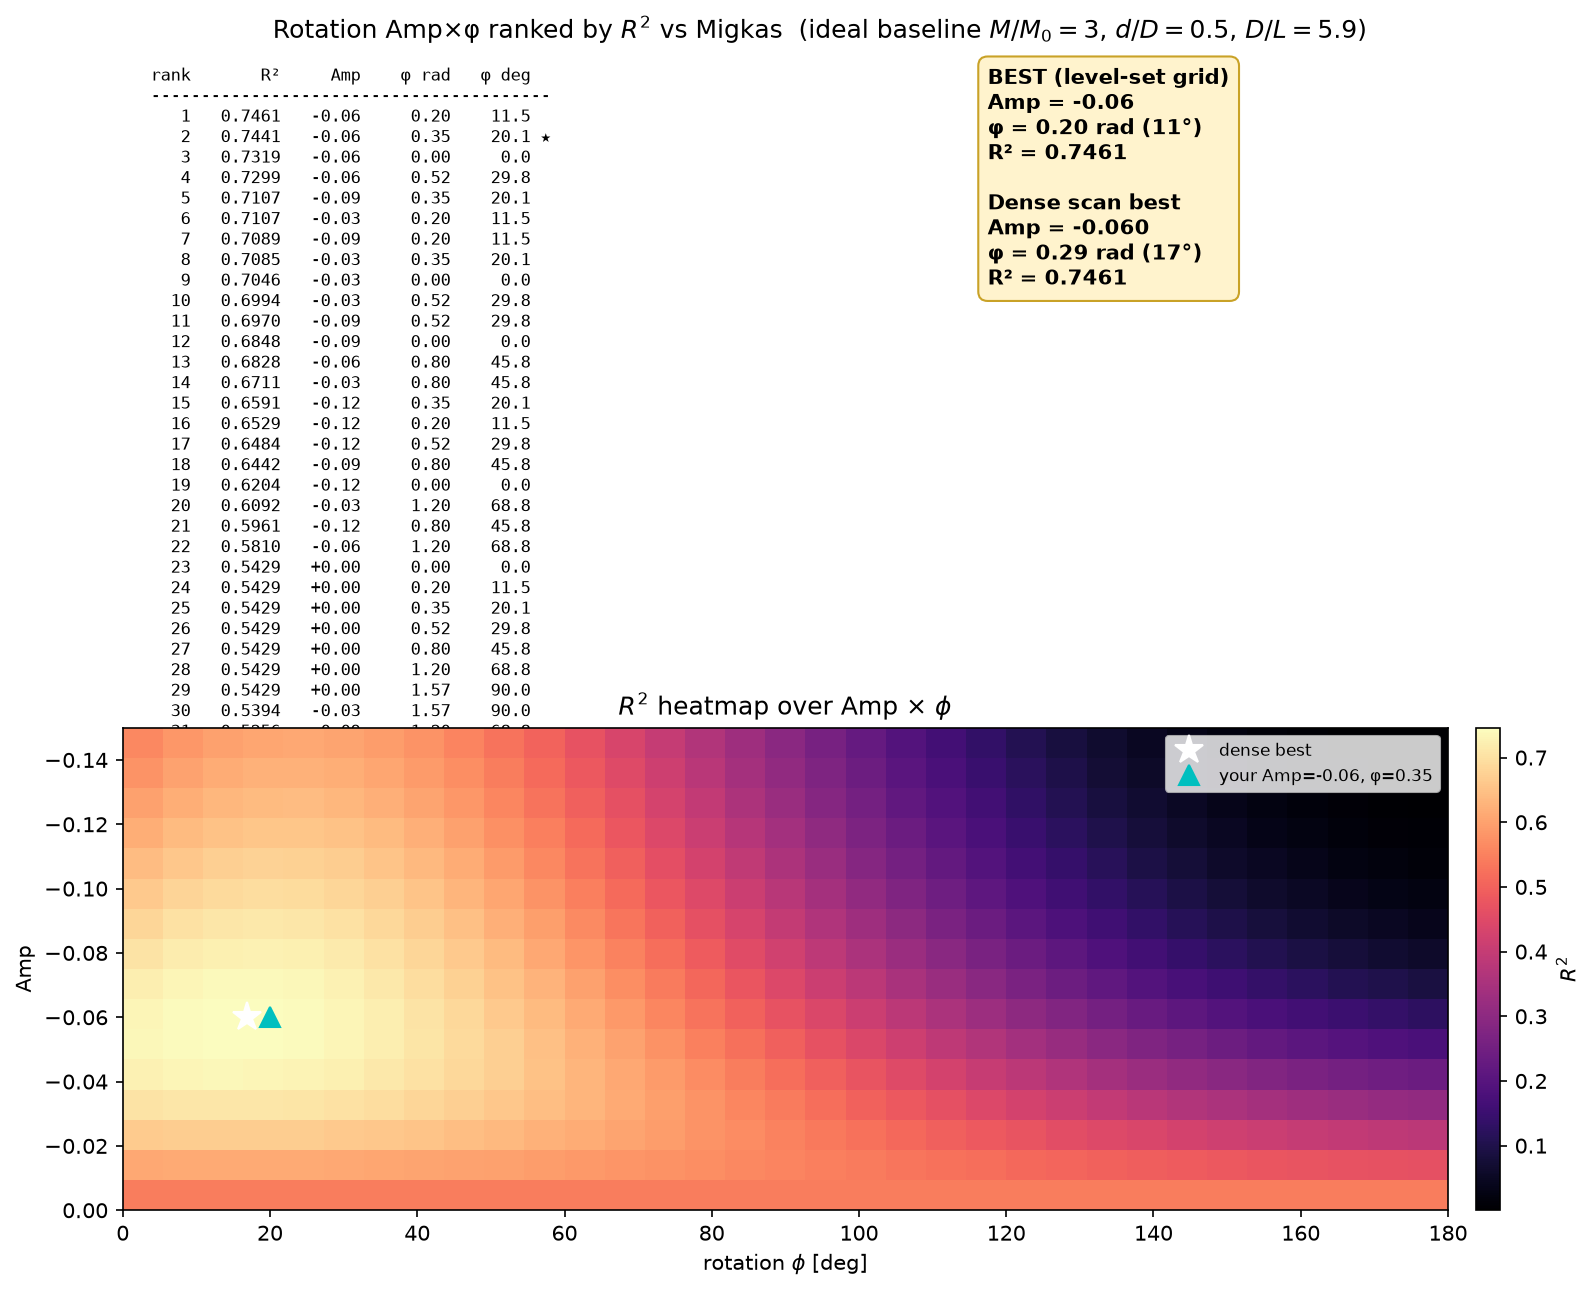
\includegraphics[width=0.95\textwidth]{rotation_Amp_phi_R2_ranked.png}
\caption{Ranked Amp$\times\phi$ $R^2$ curves.}
\label{fig:r2ranked}
\end{figure}

\begin{figure}[ht]
\centering
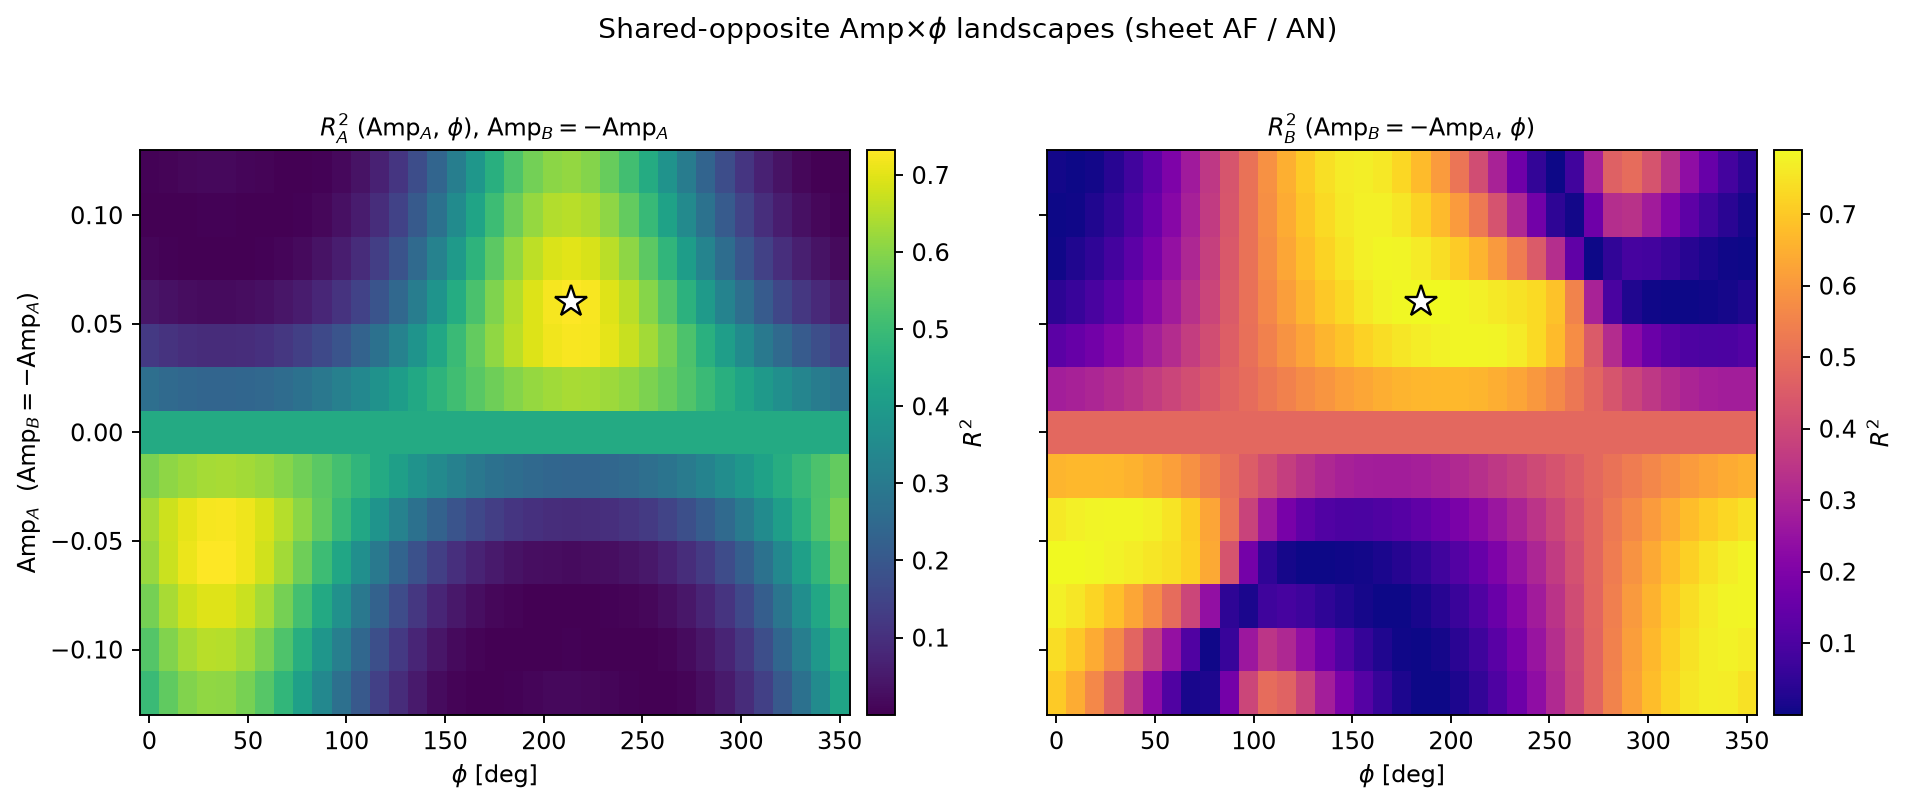
\includegraphics[width=0.95\textwidth]{rotation_Amp_phi_AB_shared_heatmaps.png}
\caption{Shared Amp$_A$/Amp$_B$ heatmaps (present on disk).}
\label{fig:sharedhm}
\end{figure}

%======================================================================
\section{Best $A$+associated $B$ / best $B$+associated $A$ with $2\ell$}
\label{sec:bestAB}

From \texttt{R2\_best\_A\_B\_Amp\_phi\_summary.csv} and the $2\ell$ npz files:

\paragraph{A-tuned.}
$\mathrm{Amp}_A=-0.06$, $\phi\approx11.5^\circ$, $\mathrm{Amp}_B=+0.06$;
$2\ell$: $\varepsilon\approx-0.043$, $\psi\approx176^\circ$;
$R^2_A\approx0.875$ (was $0.746$). Pre-$2\ell$ shared-opp $R^2_B\approx0.790$;
post-$2\ell$ associated $R^2_B$ is TBD on the summary CSV (screenshot flow
quoted $\sim0.663$).

\paragraph{B-tuned.}
$\mathrm{Amp}_B=-0.06$, $\phi\approx184.9^\circ$, $\mathrm{Amp}_A=+0.06$;
$2\ell$: $\varepsilon\approx+0.006$, $\psi\approx38^\circ$;
$R^2_B\approx0.790$, $R^2_A\approx0.766$
(\texttt{best\_fit\_2ell\_multiplier\_from\_B.npz}).

\begin{figure}[ht]
\centering
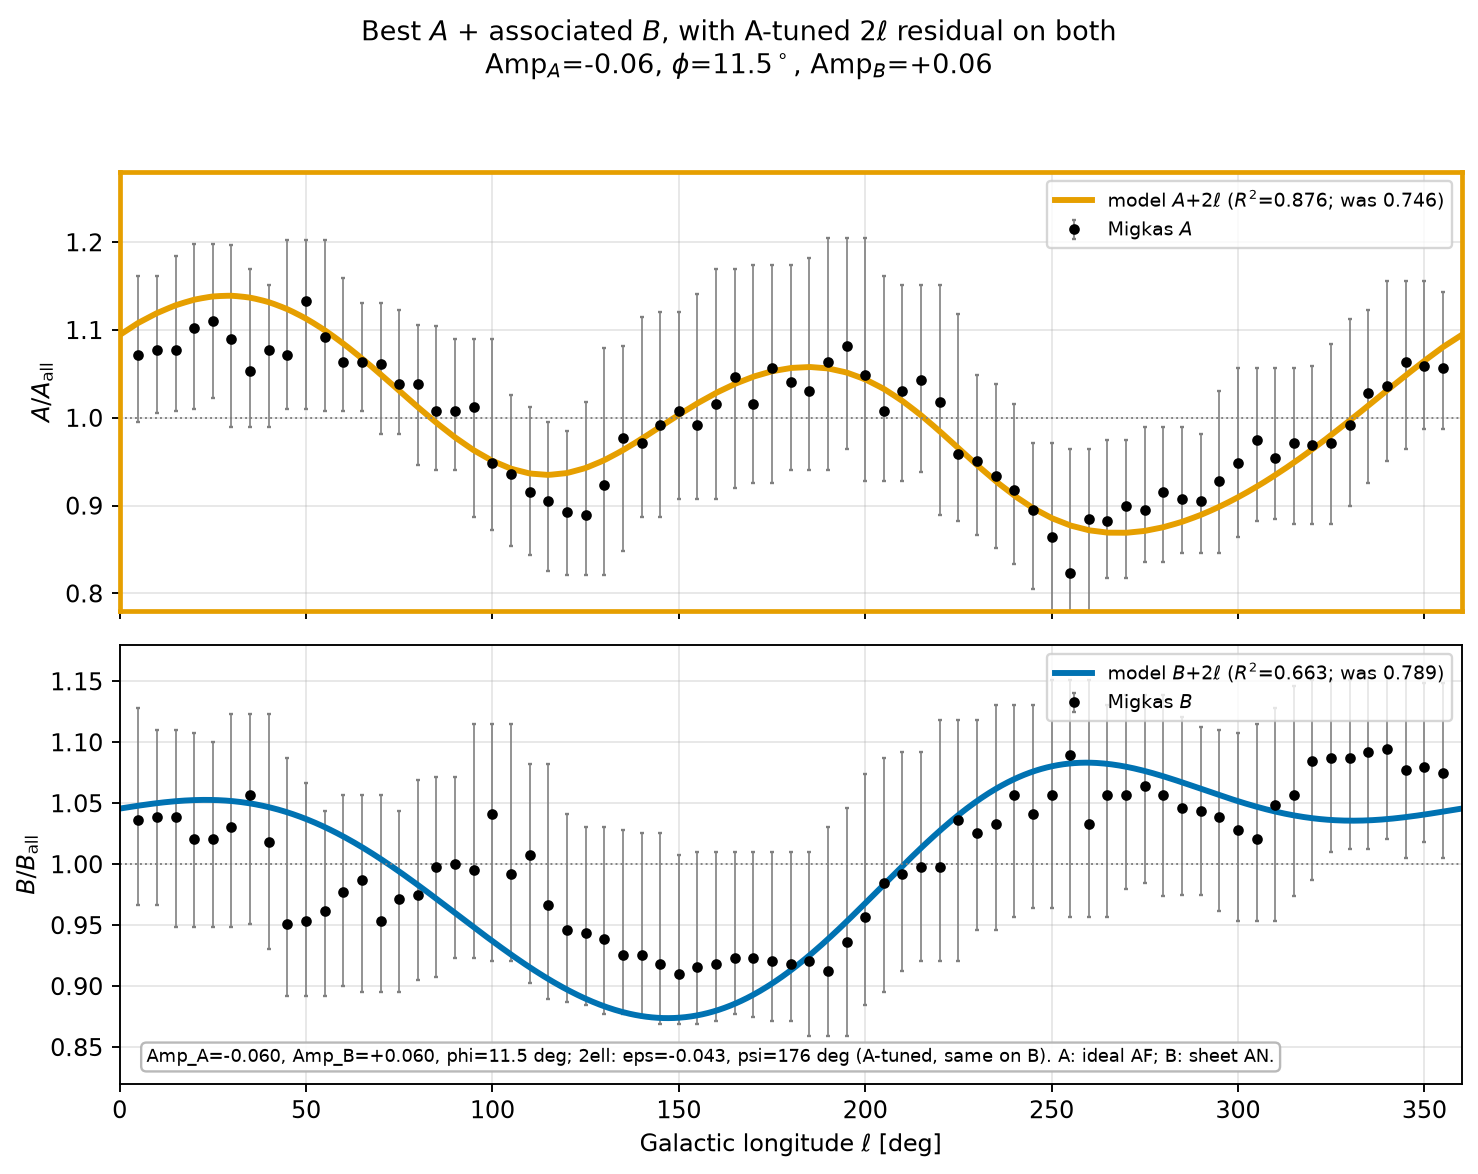
\includegraphics[width=0.92\textwidth]{best_A_vs_angle_with_associated_B_2ell.png}
\caption{Best $A$ (Amp$\times\sin$+$2\ell$) with associated $B$.}
\label{fig:bestA}
\end{figure}

\begin{figure}[ht]
\centering
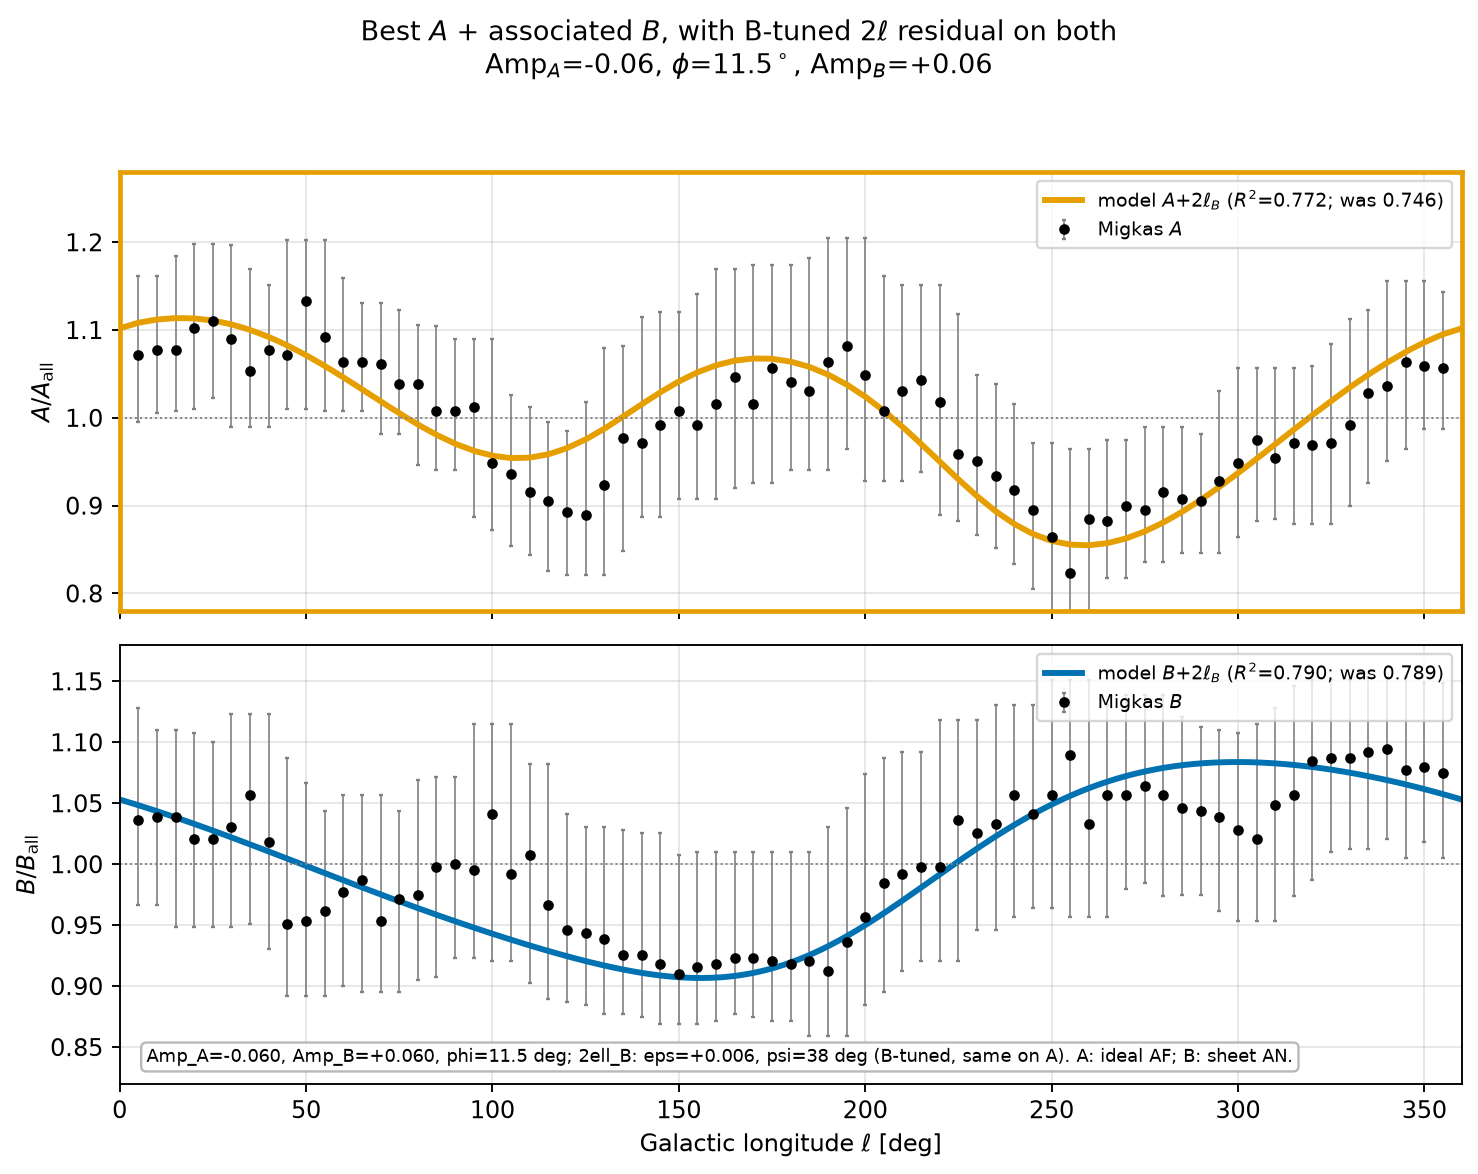
\includegraphics[width=0.92\textwidth]{best_A_vs_angle_with_associated_B_2ell_fromB.png}
\caption{Best $B$-tuned Amp$\times\sin$+$2\ell$ with associated $A$
(\texttt{\_fromB} panel).}
\label{fig:bestB}
\end{figure}

%======================================================================
\section{Amp$\times\sin$ diagnostic Mollweide family}
\label{sec:ampfamily}

Full-sky Amp$\times\sin$ diagnostic cards (physics baseline fixed; only Amp
and $\phi$ change). Not first-principles Gauss.

\begin{figure}[ht]
\centering
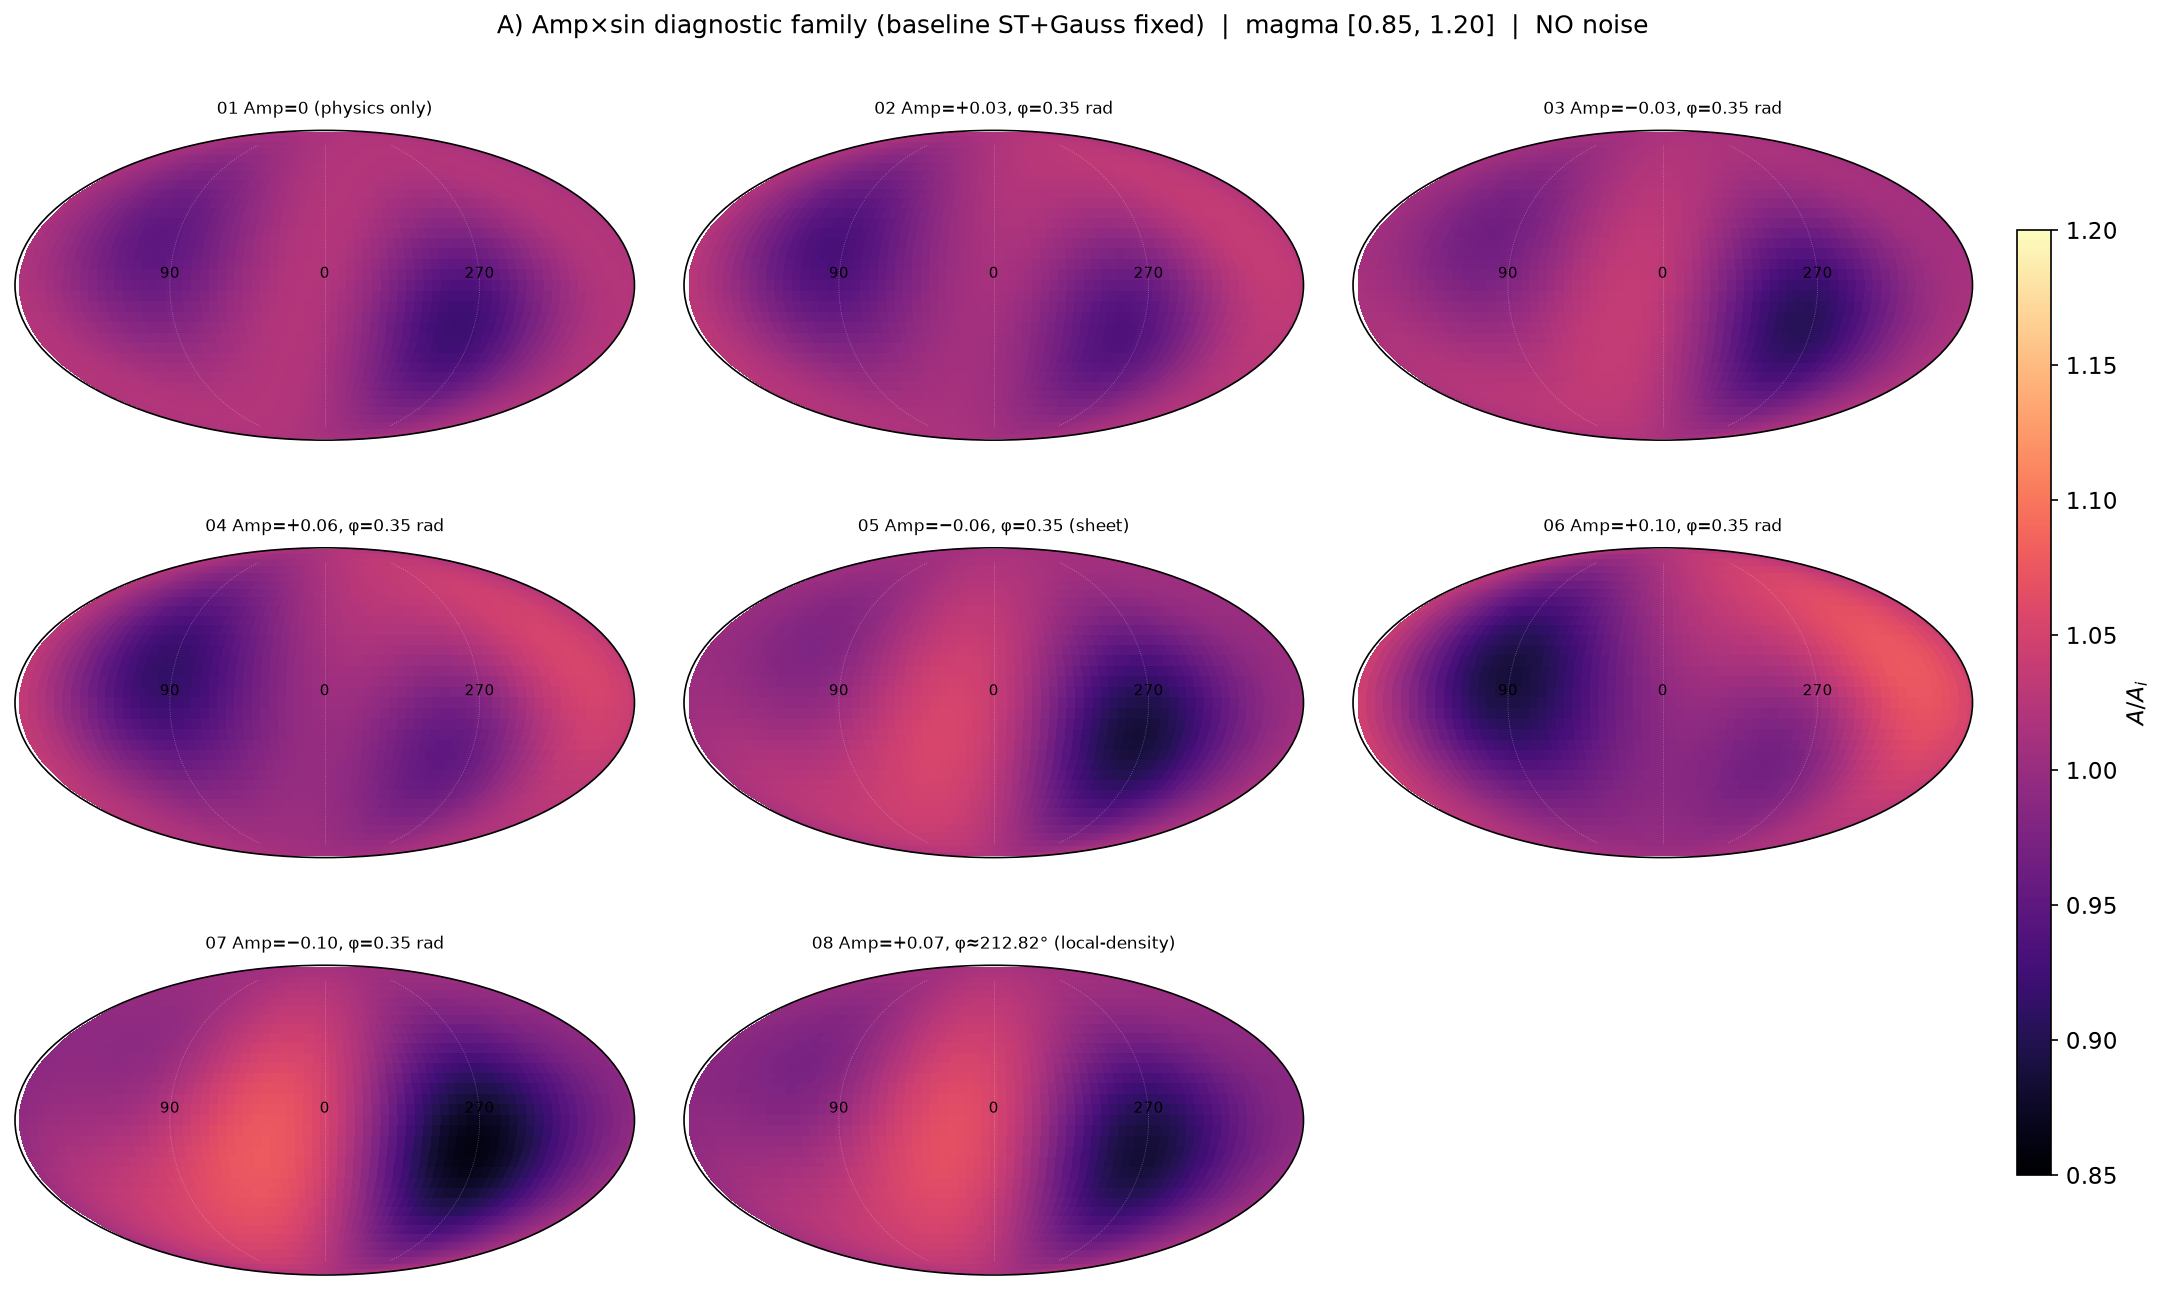
\includegraphics[width=0.98\textwidth]{GRID_amp_family.png}
\caption{Amp$\times\sin$ diagnostic Mollweide family grid.}
\label{fig:ampfamily}
\end{figure}

%======================================================================
\section{Patchwork draws}
\label{sec:patchwork}

Patchwork source map and four random draws with all markers. Fallback
filenames (\texttt{map\_09\_patchwork\_random.png},
\texttt{GRID\_patchwork\_4draws\_OWN\_EXTREMA.png} /
\texttt{\_EXTREMA.png}) exist on disk but are not needed---preferred files
are present.

\begin{figure}[ht]
\centering
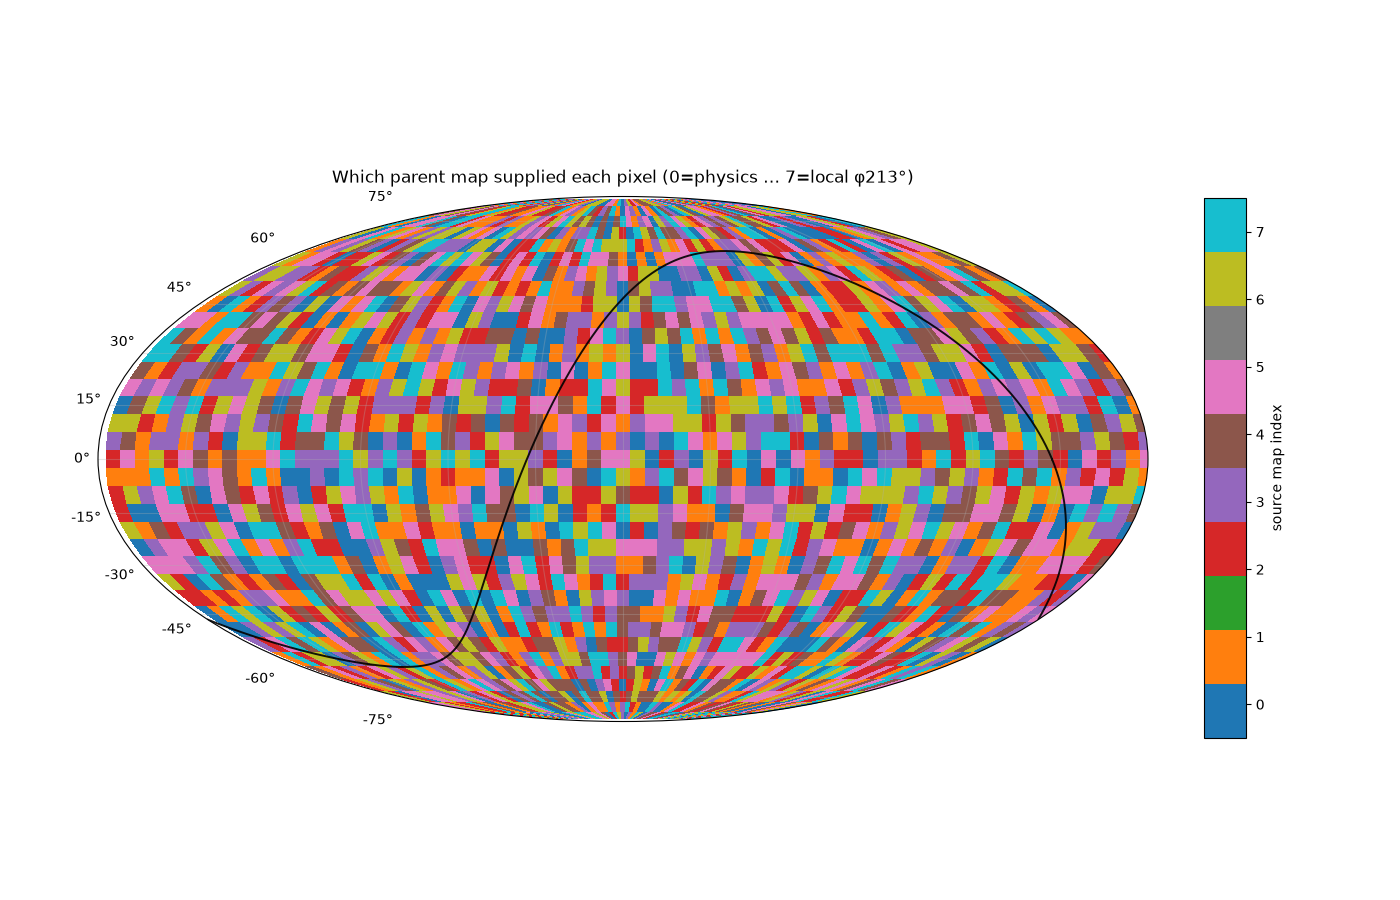
\includegraphics[width=0.92\textwidth]{map_09_patchwork_sources.png}
\caption{Patchwork sources map.}
\label{fig:patchsrc}
\end{figure}

\begin{figure}[ht]
\centering
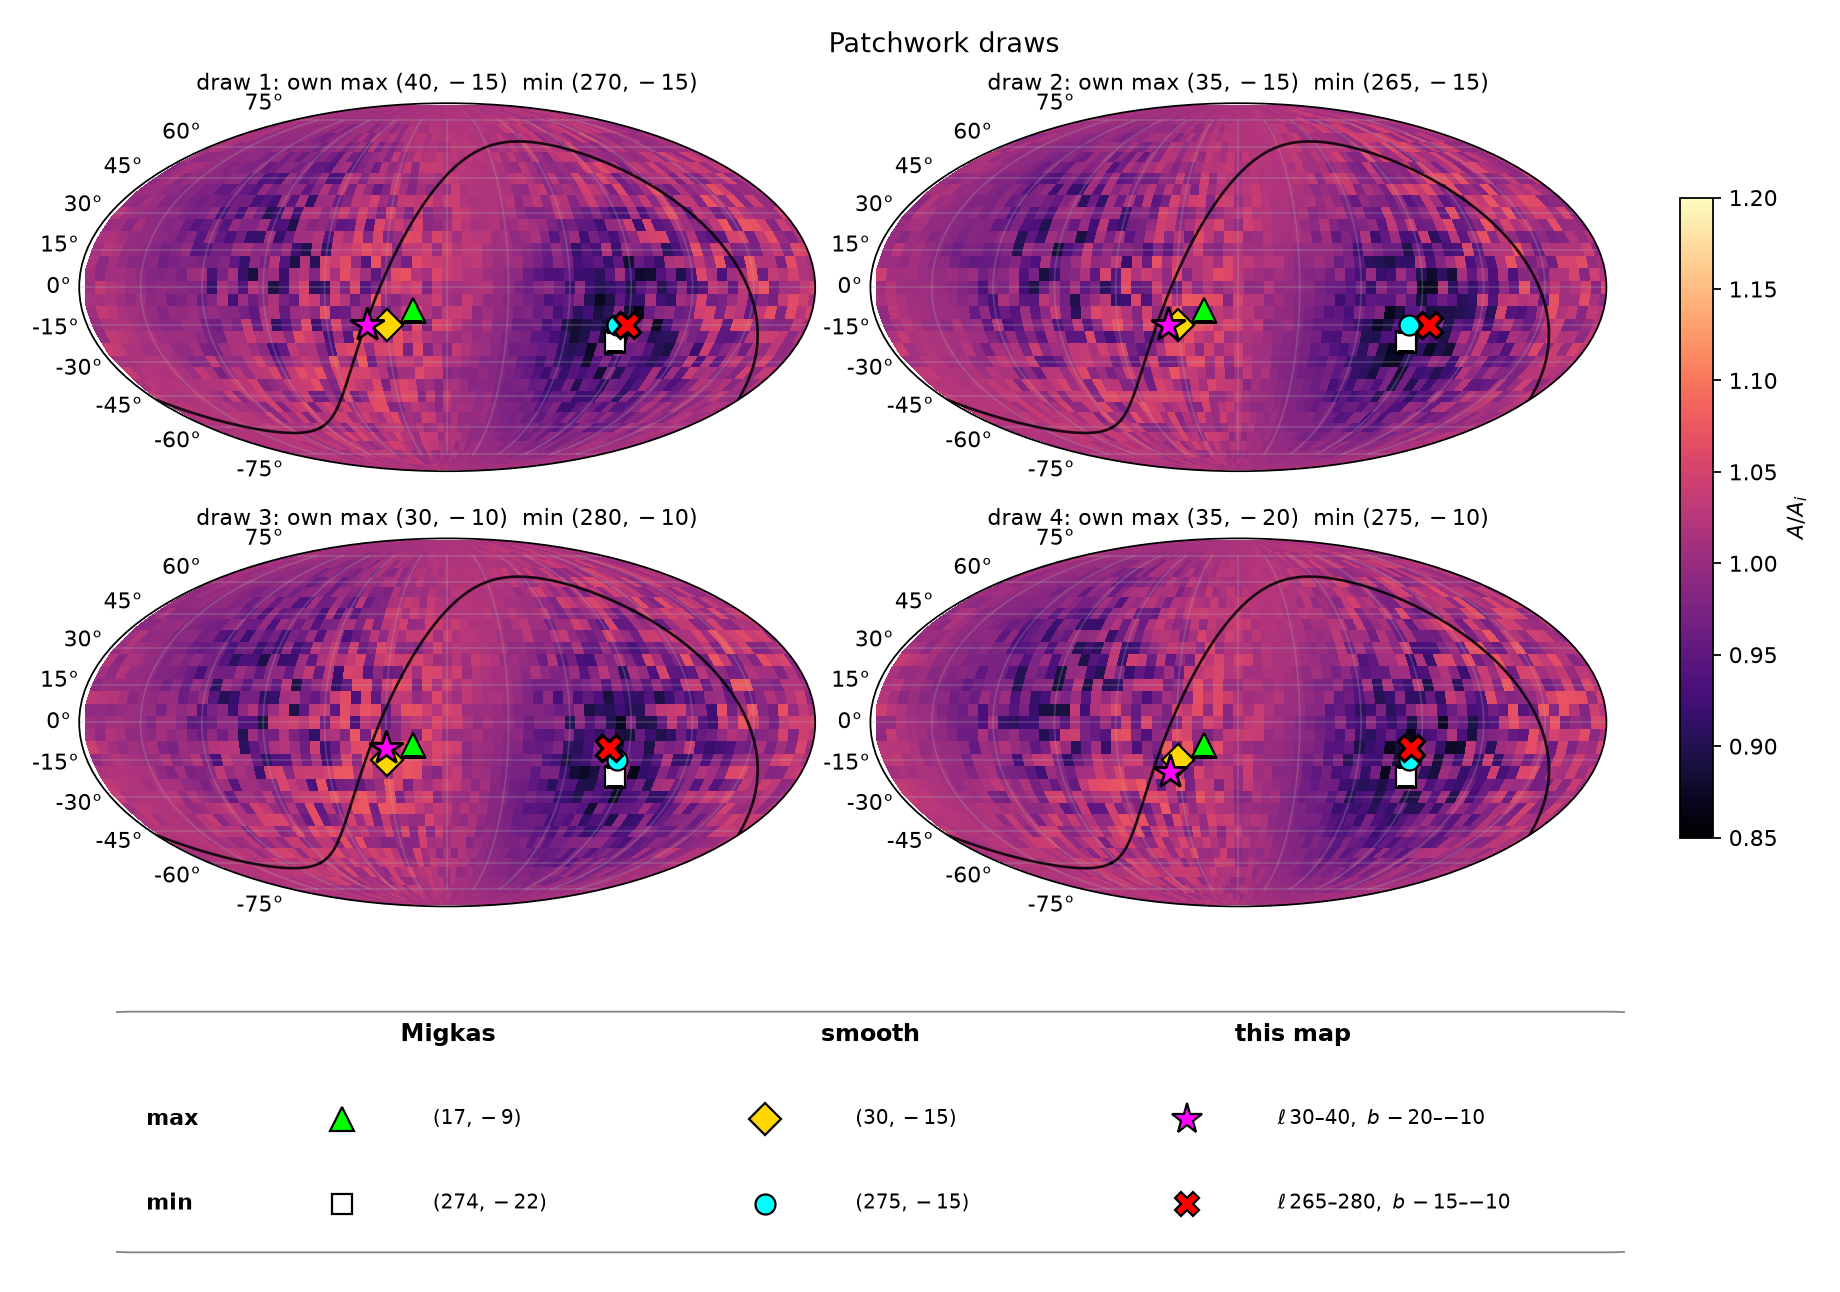
\includegraphics[width=0.98\textwidth]{GRID_patchwork_4draws_ALL_MARKERS.png}
\caption{Four patchwork draws with all markers.}
\label{fig:patchgrid}
\end{figure}

%======================================================================
\section{CMB / CoE shell schematic (deferred adversary)}
\label{sec:cmb}

Park the CMB as an open adversary. The schematic geometry: vision shell
radius $=r$; concentric shell spacing $S_n\to S_{n+1}=2r$. A blackbody-shell
dipole budget is a separate quantitative plot; this figure is only the
geometric cartoon. No closure claimed here.

\begin{figure}[ht]
\centering
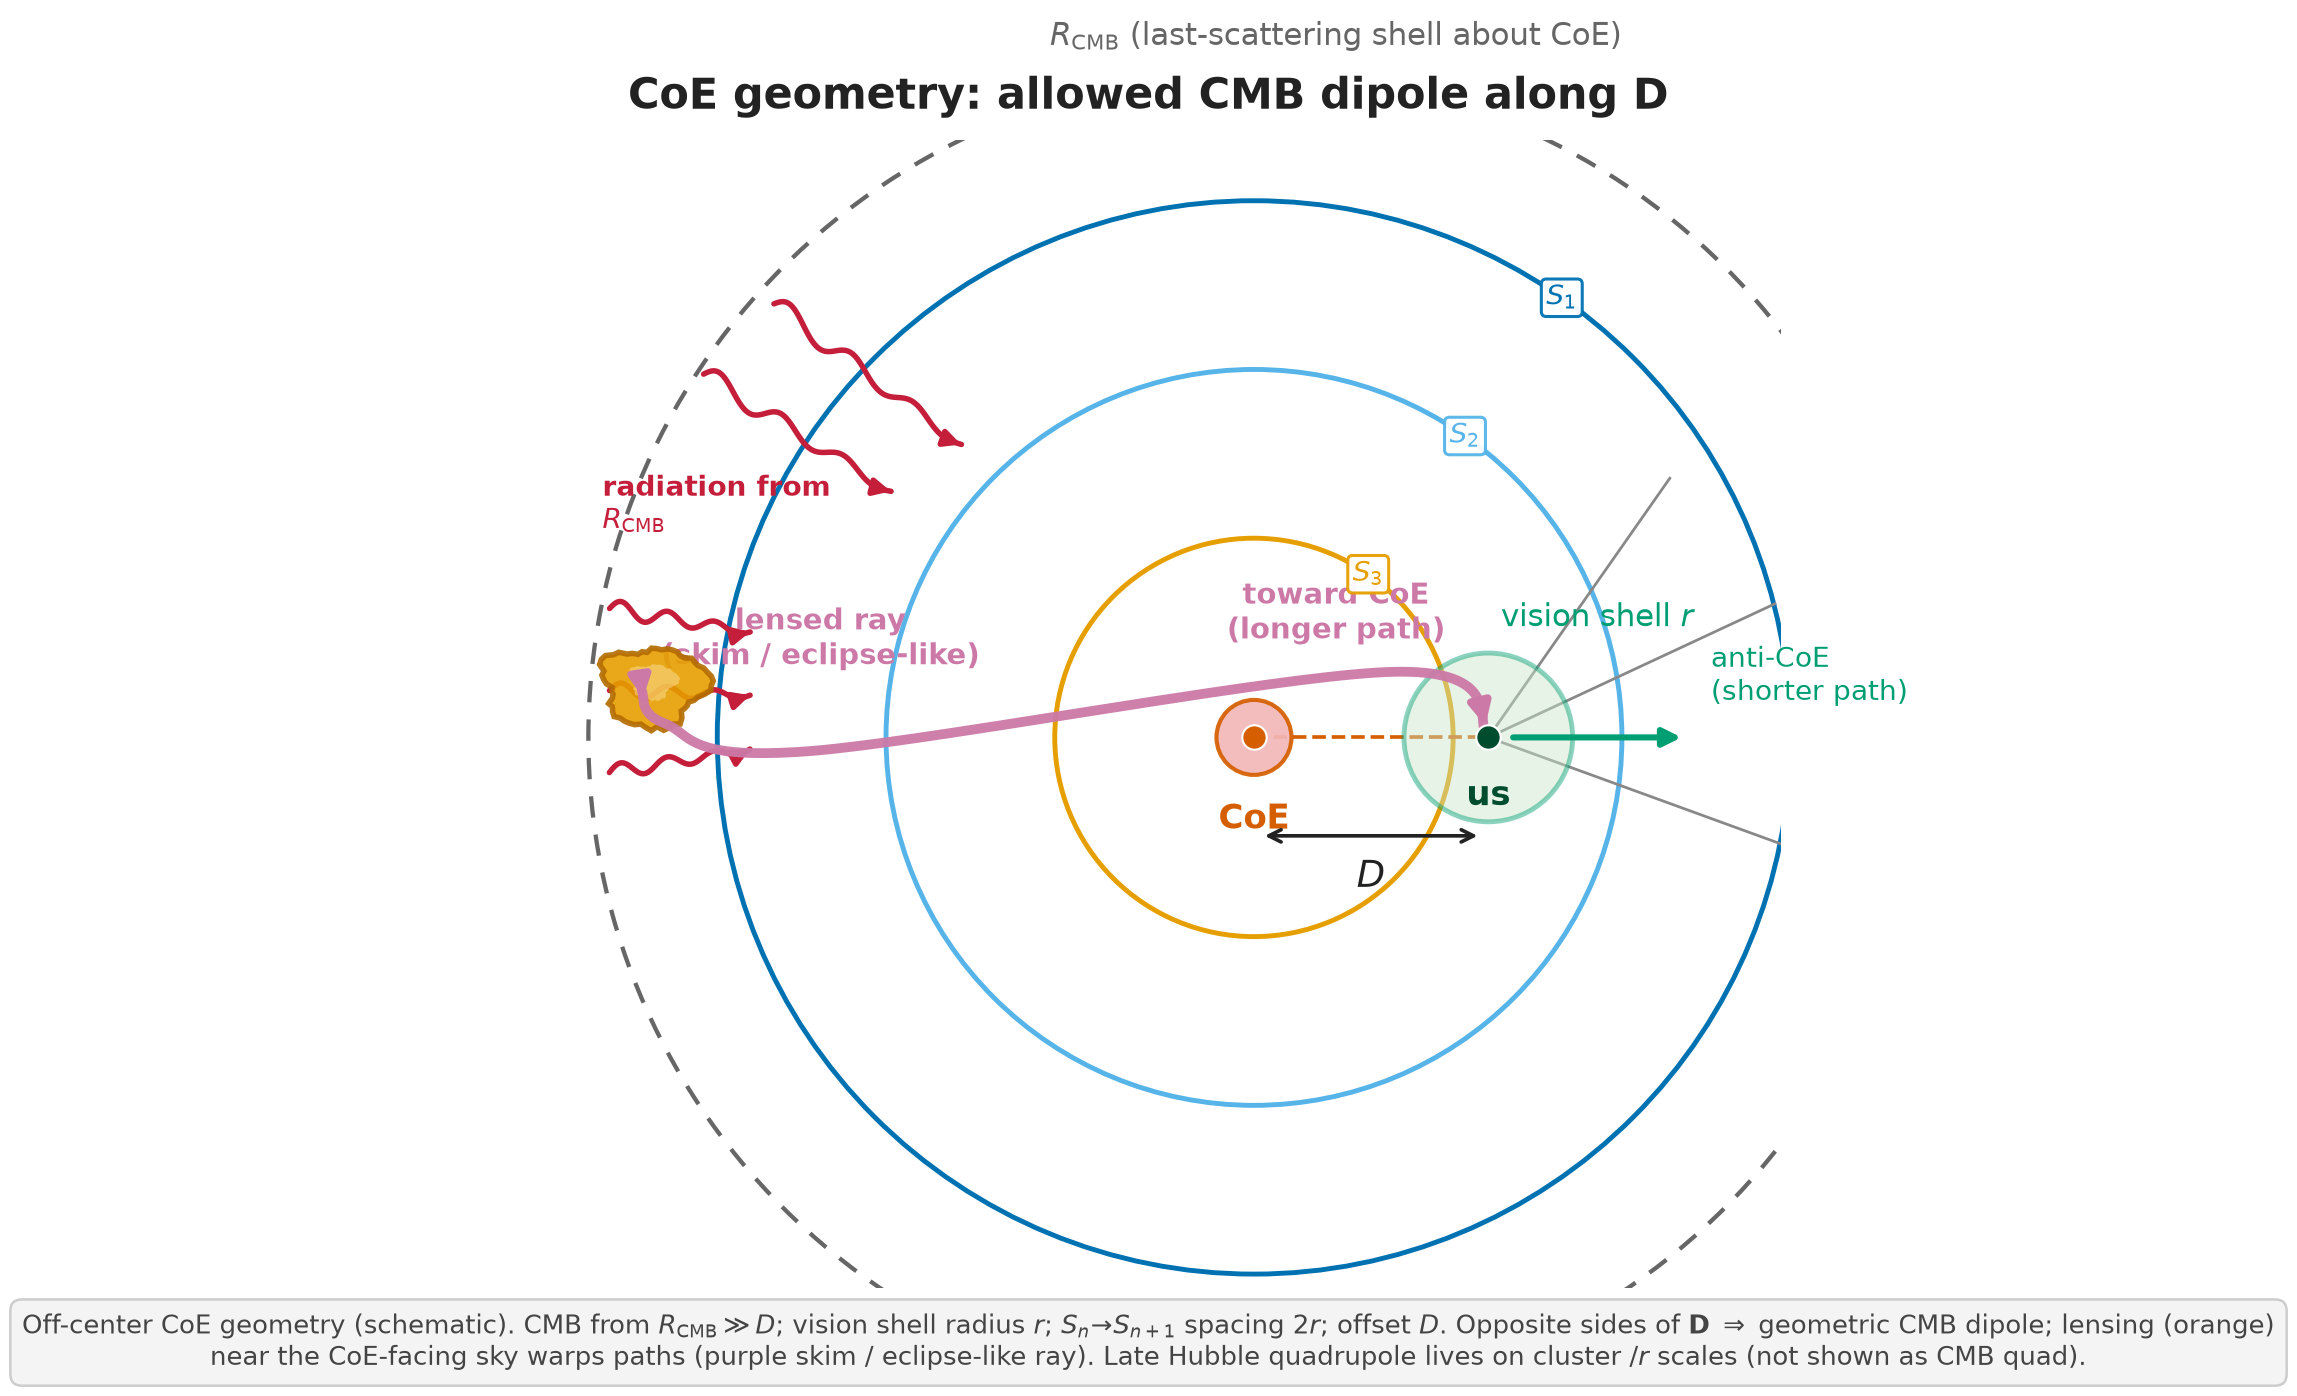
\includegraphics[width=0.92\textwidth]{coe_geometry_cmb_dipole_schematic.png}
\caption{CMB/CoE shell schematic. Vision shell radius $r$; $S_n$ to $S_{n+1}$
spacing $2r$. CMB parked as open adversary.}
\label{fig:cmb}
\end{figure}

%======================================================================
\section{Figures to add}
\label{sec:todo}

\begin{figure}[ht]
\centering
\fbox{\parbox[c][0.28\textheight][c]{0.92\textwidth}{\centering
\large\bfseries FIGURE TO ADD (1/2)\\[1em]
\rule{0.85\textwidth}{0.4pt}\\[0.5em]
\textit{Caption:}\quad\underline{\hspace{0.75\textwidth}}}}
\caption{}
\label{fig:add1}
\end{figure}

\begin{figure}[ht]
\centering
\fbox{\parbox[c][0.28\textheight][c]{0.92\textwidth}{\centering
\large\bfseries FIGURE TO ADD (2/2)\\[1em]
\rule{0.85\textwidth}{0.4pt}\\[0.5em]
\textit{Caption:}\quad\underline{\hspace{0.75\textwidth}}}}
\caption{}
\label{fig:add2}
\end{figure}

%======================================================================
\section*{Acknowledgments}
Wolfgang Rindler; Luke Ackerman (genesis).

\begin{thebibliography}{9}

\bibitem{migkas2020}
K.~Migkas, G.~Schellenberger, T.~H.~Reiprich, F.~Pacaud, M.~E.~Ramos-Ceja,
and L.~Lovisari,
\textit{Probing cosmic isotropy with a new X-ray galaxy cluster sample
through the $L_X$--$T$ relation},
arXiv:2004.03305 (2020).

\end{thebibliography}

\end{document}
